\documentclass[12pt]{spieman}  % 12pt font required by SPIE;
%\documentclass[a4paper,12pt]{spieman}  % use this instead for A4 paper
\usepackage{amsmath,amsfonts,amssymb}
\usepackage{graphicx}
\graphicspath{ {./figures/} }
\usepackage{setspace}
\usepackage{hyperref}
\usepackage{tocloft}
\usepackage{doi}
\usepackage{lineno}
\linenumbers
\usepackage{csquotes}
\MakeOuterQuote{"}
\usepackage{xr}
\externaldocument[S-]{supplementary}
\usepackage{xcolor}

\newcommand{\code}[1]{\small\texttt{#1}\normalsize}
\newcommand{\tcode}[1]{\footnotesize\texttt{#1}\normalsize}

\title{Random Matrix Theory Tools for the Predictive Analysis of Functional Magnetic Resonance Imaging Examinations}

\author[a]{Derek Berger}
\author[b,c]{Gurpreet S. Matharoo}
\author[a*,d,e,f]{Jacob Levman}

\affil[a]{St. Francis Xavier University, Department of Computer Science, 4130 University Avenue, Antigonish, Nova Scotia, Canada, B2G 2W5}
\affil[b]{St. Francis Xavier University, ACENET, 4130 University Avenue, Antigonish, Nova Scotia, Canada, B2G 2W5}
\affil[c]{St. Francis Xavier University, Department of Physics, 4130 University Avenue, Antigonish, Nova Scotia, Canada, B2G 2W5}
\affil[d]{Athinoula A. Martinos Center for Biomedical Imaging, 149 Thirteenth Street, Suite 2301, Charlestown, Massachusetts, United States, 02129}
\affil[e]{Harvard Medical School, Department of Radiology, 25 Shattuck Street Boston, Massachusetts, United States, 02115}
\affil[f]{Nova Scotia Health Authority, Research Affiliate, Nova Scotia, Canada}


\renewcommand{\cftdotsep}{\cftnodots}
\cftpagenumbersoff{figure}
\cftpagenumbersoff{table}
\begin{document}
\maketitle

\begin{abstract}

\section*{Purpose}
Random matrix theory (RMT) is an increasingly useful tool for understanding
large, complex systems. Prior studies have examined functional Magnetic
Resonance Imaging (fMRI) scans using tools from RMT, with some success.
However, RMT computations are highly sensitive to a number of analytic choices,
and the robustness of findings involving RMT remain in question. We
systematically investigate the usefulness of RMT on a wide variety of fMRI
datasets using a rigorous predictive framework.

\section*{Approach}
We develop open-source software to efficiently compute RMT features from fMRI
images, and examine the cross-validated predictive potential of eigenvalue and
RMT-based features (``eigenfeatures'') with classic machine-learning
classifiers. We systematically vary pre-processing extent, normalization
procedures, RMT unfolding procedures, and feature selection, and compare the
impact of these analytic choices on the distributions of cross-validated
prediction performance for each combination of dataset binary classification
task, classifier, and feature. To deal with class imbalance, we use the
area under the receiver operating characteristic curve (AUROC) as the main
performance metric.

\section*{Results}
Across all classification tasks and analytic choices, we find RMT- and
eigenvalue-based "eigenfeatures" to have predictive utility more often than
not (82.4\% of median AUROCs \(>\) 0.5; median AUROC range across
classification tasks 0.47 - 0.64). Simple baseline reductions on source
timeseries, by contrast, were less useful (58.8\% of median AUROCs \(>\) 0.5,
median AUROC range across classification tasks 0.42 - 0.62). Additionally,
eigenfeature AUROC distributions were overall more right-tailed than
baseline features, suggesting greater predictive potential. However, performance
distributions were wide, and often significantly affected by analytic choices.


\section*{Conclusions}
Eigenfeatures clearly have potential for understanding fMRI functional
connectivity in a wide variety of scenarios. The utility of these features is
strongly dependent on analytic decisions, suggesting caution when interpreting
past and future studies applying RMT to fMRI. However, this study demonstrates
that the inclusion of RMT statistics in fMRI investigations could improve
prediction performances across a wide variety of phenomena.

\end{abstract}

\keywords{random matrix, spectral rigidity, level number variance, fMRI, classification, machine-learning}

{
\noindent
\footnotesize
\textbf{*}Jacob Levman,  \linkable{jlevman@stfx.ca}
(primary), \linkable{jlevman@mgh.harvard.edu}
}

\begin{spacing}{2}

\section{Introduction}
\label{sect:intro}

\color{cyan}

At its most rudimentary, the basic insight of Random Matrix Theory (RMT) is
that matrices can be described by their eigenvalues, and that
large matrices (or large collections of matrices) can be
well-described by the statistical behaviour of those eigenvalues. Such a
description is obtained by assuming that the large matrix (or collection
of matrices) is sampled from a \textit{class} or \textit{ensemble} of random
matrices.

Simplifying somewhat, a random matrix is a matrix that has entries that can be
well-described as being drawn from a particular independent and identically
distributed (\textit{iid}) distribution, or, equivalently, is a matrix where
each entry is itself a random variable. A \textit{class} or \textit{ensemble}
of random matrices is generally defined by the shape of the \textit{iid}
distribution involved. For example, the Gaussian Orthogonal Ensemble (GOE) is a
\textit{class} or \textit{ensemble} of random matrices that comprises
orthogonal matrices with each entry being sampled from a standard Gaussian, and
the Marchenko-Pastur distribution describes the limiting behaviour of the
singular values of \textit{iid} rectangular random matrices where the
\textit{iid} distribution is arbitrary\cite{mehtaRandomMatrices2004}. Of
course, given a single particular matrix, one can only estimate a
\textit{probability} that it is a member of a certain class, since certain RMT
classes can yield arbitrary matrices (albeit with extremely low probability).


and eigenvalue distributions of GOE random matrices have a
number of well-understood properties\cite{mehtaRandomMatrices2004,
guhrRandommatrixTheoriesQuantum1998a}. Even more generally,



Specifically, RMT finds that often, in the infinite limit, that the expected
distribution of the eigenvalues of a number of classes of random matrices can
be described quite precisely.\cite{andersonIntroductionRandomMatrices2010,
akemannOxfordHandbookRandom2011, mehtaRandomMatrices2004}. Although these
assumptions are quite specific and restrictive, nevertheless, RMT-predicted
eigenvalue distributions have appeared in diverse natural phenomena.

\color{black}


\textcolor{cyan}{Thus, while} first developed to describe the fluctuation of nuclei
energy levels in quantum physics \cite{mehtaRandomMatrices2004,
guhrRandommatrixTheoriesQuantum1998a}, RMT has been shown to have extremely
broad potential. In small-scale physical systems, RMT universalities have been
observed in quantum chaotic systems, complex nuclei, atoms, molecules and
disordered mesoscopic systems \cite{guhrRandommatrixTheoriesQuantum1998a,
mehtaRandomMatrices2004, brodyRandommatrixPhysicsSpectrum1981,
beenakkerRandommatrixTheoryQuantum1997,
bohigasHigherOrderCorrelationsSpectra1985, wintgenLevelStatisticsQuantized1988,
pandeySkewOrthogonalPolynomialsUniversality2001}, and at larger scales, RMT has
been applied to atmospheric physics
\cite{santhanamStatisticsAtmosphericCorrelations2001}, stock cross-correlations
\cite{plerouRandomMatrixApproach2002}, social networks
\cite{jalanUncoveringRandomnessSuccess2014}, random networks
\cite{bandyopadhyayUniversalityComplexNetworks2007}, network-formation in
liquids\cite{sastrySpectralStatisticsInstantaneous2001,
matharooSpectralStatisticsQuenched2009} and amorphous clusters
\cite{sarkarUniversalityVibrationalSpectra2004,
matharooVibrationalSpectraAmorphous2005,
matharooUniversalityVibrationalSpectra2008}. Within biological systems, RMT has
also been used to successfully model aspects of  amino acid functional
relationships \cite{bhadolaTargetingFunctionalMotifs2016}, synchrony in
epileptic seizures \cite{osorioPhasesynchronizationRandommatrixBased2011}, and
in protein-protein interactions both in different species
\cite{agrawalQuantifyingRandomnessProtein2014} and breast cancer
\cite{raiRandomnessPreservedPatterns2015}. RMT has also been used to guide
statistical decisions in principal components
analyses\cite{franklinParallelAnalysisMethod1995,
veraartDenoisingDiffusionMRI2016, ulfarssonDimensionEstimationNoisy2008}, and,
more recently, has provided insights into the behaviors of deep neural
networks\cite{martinImplicitSelfRegularizationDeep2021,
martinPredictingTrendsQuality2021}.

\textcolor{orange}{When or if RMT has} real-world explanatory potential,
\textcolor{orange}{this will most likely be} when dealing with a complex system
of many (hundreds or more\cite{mehtaRandomMatrices2004}) interacting
components, \textcolor{orange}{rather than a system that is too small for
statistical regularities ro reliably surface}. If such a system has a matrix
representation, and the eigenvalues of this representation have a distribution
similar to one predicted by RMT, it suggests the system is either highly random
or chaotic. By contrast, if the observed spectra deviate significantly from
RMT-predicted spectra, this
suggests otherwise. A number of studies have used RMT to make such
interpretations and comparisons between
systems\cite{santhanamStatisticsAtmosphericCorrelations2001,
jalanUncoveringRandomnessSuccess2014,
bandyopadhyayUniversalityComplexNetworks2007,
agrawalQuantifyingRandomnessProtein2014, raiRandomnessPreservedPatterns2015,
sebaRandomMatrixAnalysis2003, wangSpectralPropertiesTemporal2015,
wangRandomMatrixTheory2016, matharooSpontaneousBackpainAlters2020}.

\subsection{RMT and Neurobiological Signals}

In the human brain, each neuron, collection of neurons, or region of interest
(ROI) is a potentially-interacting component in a complex system. RMT
may have potential in describing the totality of these interactions, provided
that measurements of functioning can be obtained with sufficient spatial and
temporal resolution to speak to some neurobiological or neuropsychological
phenomenon of interest.

For an imaging modality like fMRI, where changes in the
blood-oxygenation-level-dependent (BOLD) signals are related to neural
activity, RMT may be an ideal starting point, as each voxel time course (or
collection of such time sources, i.e. ROIs) can be considered an interacting
component of the system. Likewise, in functional connectivity
analyses, statistical relationships of the BOLD ROI time-courses are
investigated in the hope of gaining insights into brain function (see
\citenum{bastosTutorialReviewFunctional2016,
vandenheuvelExploringBrainNetwork2010} for reviews, but also
\citenum{nobleDecadeTestretestReliability2019} and
\citenum{lurieQuestionsControversiesStudy2020} for challenges facing functional
connectivity analyses). In this framework, each connection or correlation can
be considered a system component, and the eigenvalues of such a correlation
matrix can be examined from the perspective of RMT.

The earliest study taking this approach demonstrated that spectra of the
correlations between electroencephalographic (EEG) signals closely resemble
those of the Gaussian Orthogonal Ensemble (GOE)
\cite{sebaRandomMatrixAnalysis2003}. In fMRI, RMT has been used to evaluate the
quality of whole brain features extracted from fMRI data
\cite{voultsidouFeatureEvaluationFMRI2007, verganiRestingStateFMRI2019}, and in
diffusion MRI to aid in the selection of the number of components to employ in
principal-component reduction analysis and denoising
\cite{veraartDenoisingDiffusionMRI2016, verganiRestingStateFMRI2019,
ulfarssonDimensionEstimationNoisy2008}.

RMT has also been used in ROI-based fMRI functional connectivity studies to
investigate differences between rest and task states
\cite{wangSpectralPropertiesTemporal2015}, between subjects with and without
attention-deficit hyperactive disorder (ADHD)
\cite{wangRandomMatrixTheory2016}, between pain and non-pain states
\cite{matharooSpontaneousBackpainAlters2020}, and between left-sided vs. \
right-sided motor imagery \cite{guRandomMatrixTheory2020}. While no differences
were found in the latter study, across the first three studies, the spectra of
resting or low-attention states exhibited properties close to the GOE. These
findings suggest that certain aspects of psychological processes might be
characterized, in part, by features computed from the eigenvalues of fMRI
correlation matrices, and that these features might vary in an interpretable
manner across psychological processes. If this is the case, RMT could aid in
understanding the functioning of the human brain.


\subsection{Eigenvalue Features}

The basic insight of RMT is thus that eigenvalues alone may provide
interesting information about highly complex systems. However, real systems are
usually noisy, and involve a mixture of random and non-random components and
interactions. RMT is statistical in nature, describing only the expected
behavior of the spectra of \textit{iid} random matrices. To this end, a number
of summary statistics or ``spectral observables''
\cite{mehtaRandomMatrices2004, guhrRandommatrixTheoriesQuantum1998a} can be
computed from empirically observed spectra, with these spectral observables
sometimes being better suited for further analysis, or for the comparison of
empirical observations to theory. Two such summary statistics that have been
popular\cite{santhanamStatisticsAtmosphericCorrelations2001,
jalanUncoveringRandomnessSuccess2014, matharooSpontaneousBackpainAlters2020,
bandyopadhyayUniversalityComplexNetworks2007,
agrawalQuantifyingRandomnessProtein2014, raiRandomnessPreservedPatterns2015,
sebaRandomMatrixAnalysis2003,wangSpectralPropertiesTemporal2015,
wangRandomMatrixTheory2016} are the \textit{spectral rigidity} and
\textit{level number variance} (``rigidity'' and ``level variance'' for short;
details in Section \ref{sec:methods}).

However, from a predictive standpoint, these summary statistics may
\textcolor{orange}{mask} predictively-useful information. If the basic RMT
insight is that the eigenvalues alone can provide understanding of a system,
then those eigenvalues (or other simple transformations of them) ought also to
be predictively useful.
We examine a number of such features in this study, and refer to both
RMT-derived features like the rigidity and level variance, and non-RMT-derived
features collectively as \textit{eigenfeatures} in this study.

\subsection{Functional Connectivity Reduction}

The functional connectivity—often, the matrix of correlations of
various collections of voxels of an fMRI scan—is \textit{a priori} a useful
representation of the fMRI data. However, the full correlation matrix between
all voxels is itself often computationally infeasible to work with, and thus is
reduced in various ways prior to being used in analyses.

Typical reductions include the use of a ``seed'' voxel or collection of voxels
(see e.g. \citenum{joelRelationshipSeedbasedICAbased2011,
smithCharacterizingIndividualDifferences2014}): the mean signal over that ROI
is correlated with all other \(N\) ROIs of interest to generate a reduced
functional connectivity matrix (or image) with one correlation value at each
non-seed ROI. This sort of reduction reduces the functional connectivity to
\(N\) values, but necessarily biases the analysis to the seed ROI.

Likewise, one can work with ROI mean signal reductions, or independent
component analysis reductions\cite{joelRelationshipSeedbasedICAbased2011,
smithCharacterizingIndividualDifferences2014}, and work with the \(N \times N\)
matrix of the correlations of these reductions. This analysis is, \textit{a
priori}, sensitive to the choice of ROIs, and, in the case of anatomical
atlases / parcellations for ROIs, may also lack theoretical justification.

RMT suggests a potentially useful reduction in the form of the eigenvalues of
the voxelwise functional connectivity \textcolor{orange}{matrix}. An \(N \times
t\) matrix of \(N\) time series of length \(t\), and where \(t \ll N\) will
have a symmetric correlation (or covariance) matrix with \(t - 1\) non-zero,
positive real-valued eigenvalues. These eigenvalues can be computed highly
efficiently via transposition of the voxelwise correlation or covariance
matrix.

\subsection{Limitations of Previous Work}

Previous studies applying RMT to functional connectivity
data\cite{wangRandomMatrixTheory2016, wangSpectralPropertiesTemporal2015a,
matharooSpontaneousBackpainAlters2020, guRandomMatrixTheory2020} took largely
descriptive / explanatory approaches, noting only differences in RMT across
subgroups and/or conditions. For example Wang et al.
(2016)\cite{wangRandomMatrixTheory2016} and Gu et al.
(2020)\cite{guRandomMatrixTheory2020} use a Kolmogorov-Smirnov test, and Wang
et al. (2015)\cite{wangSpectralPropertiesTemporal2015a} uses a t-test to
provide evidence of differences in various RMT metrics. However, statistically
significant differences in a metric do not necessarily imply practical
significance or predictive utility \cite{loWhySignificantVariables2015}, nor do
they imply generalization or replicability \cite{amrheinEarthFlat052017}.
Cross-validation, by contrast, attempts to more directly assess these
properties \cite{yarkoniChoosingPredictionExplanation2017}.

In addition, the previous papers do not provide publicly-accessible code to
reproduce results. The extraction of the spectral rigidity and level variance
is computationally-demanding and mathematically and algorithmically
non-trivial, and additionally requires an \textit{unfolding}
procedure\cite{guhrRandommatrixTheoriesQuantum1998a, mehtaRandomMatrices2004}.
Unfolding is an exponential fitting procedure that involves a number of highly
subjective decisions regarding outliers and the flexibility of the fitting
function. These decisions are, unfortunately, often poorly
\textcolor{orange}{documented} or even entirely \textcolor{orange}{missing from
method descriptions, despite being} known to often dramatically impact RMT
conclusions \cite{abul-magdUnfoldingSpectrumChaotic2014,
abueleninSpectralUnfoldingChaotic2018, fossionRandommatrixSpectraTime2013,
abueleninEffectUnfoldingSpectral2012, moralesImprovedUnfoldingDetrending2011}.

In addition to the flexibility in the implementation and application of RMT to
empirical data, there is also flexibility introduced by analytic choices made
in the complex preprocessing pipelines of
fMRI\cite{parkerBenefitSliceTiming2019}. These "researcher degrees of
freedom"\cite{simmonsFalsePositivePsychologyUndisclosed2011b}, in combination
with the absence of reproducible code and data availability, and predominance
of descriptive and explanatory approaches, \textcolor{orange}{may} raise doubts about the basic
robustness and practical utility of \textcolor{orange}{past} RMT-based functional connectivity analyses.

What is missing is a rigorous, systematic, reproducible investigation of the
predictive value of RMT metrics across a wide variety of data, analytic
choices, RMT features, and preprocessing decisions, with RMT features being
compared to simpler alternative baseline predictors. The current study aims to
remedy this.


\section{Datasets}
\label{sec:datasets}

\subsection{Overview}

We selected fMRI data publicly available on the
\href{https://openneuro.org/}{OpenNeuro}
platform\cite{markiewiczOpenNeuroResourceSharing2021}. Selection criteria was
somewhat subjective, but we required each dataset to (1) comprise 10 or more
human subjects, (2) have all fMRI \textcolor{orange}{runs} have the same
spatial and temporal resolutions, (3) have fMRI images that can be split into
various classes for a number of binary classification tasks, and (4), allow
reasonably classifying each run \textcolor{orange}{using all of the run 4D
voxel data only.} \textcolor{cyan}{That is, for this last point, classification
of a run should be reasonable in the absence of run-specific task or event
timings or details, and should not require using only some subset of the total
set of 3D volumes (e.g. those associated only with some task or event
timings)}. This yielded seven datasets total.


\begin{table}[h!]
\caption{
    \label{tab:data-dimensions}
    Included fMRI dataset details.
    Name = Identifier for paper.
    Dimensions listed as M x N x P, indicate P axial slices each with dimensions M x N.
    TR = Time of Repetition (seconds).
    \textcolor{orange}{Volumes = Number of 3D volumes per run.}
    n\_scans = Total number of \textcolor{orange}{4D images in dataset (number of subjects times number of runs per subject)}.
}
\small
\centering
\begin{tabular}{ l c c c c c c }
\hline
\textbf{Name}    & \textbf{Dimensions}  & \textbf{Voxel size (mm)} & \textbf{TR} & \textbf{Volumes} & \textbf{n\_scans} \\
\hline
Aging     & 74 × 74 × 32   & 3.0 × 3.0 × 4.0 & 2.0  & 300 & 62  \\
Bilingual    & 100 × 100 × 72 & 1.8 × 1.8 × 1.8 & 0.88 & 823 & 90  \\
Depress   & 112 × 112 × 25 & 2.0 × 2.0 × 5.0 & 2.5  & 100 & 72  \\
Learn     & 64 × 64 × 36   & 3.0 × 3.0 × 3.0 & 2.0  & 195 & 432 \\
Osteo     & 64 × 64 × 36   & 3.4 × 3.4 × 3.0 & 2.5  & 300 & 74  \\
Park      & 80 × 80 × 43   & 3.0 × 3.0 × 3.0 & 2.4  & 149 & 552 \\
Attention & 128 × 128 × 70 & 1.5 × 1.5 × 1.5 & 3.0  & 300 & 90  \\
\hline
\end{tabular}
\end{table}

In order not to inundate readers with dataset details, and because this is an
exploratory investigation of RMT which is not committed to any specific
theory\footnote{In fact, datasets and, later, the classification tasks, were
chosen without investigation into any findings or publications associated with
the data, both in order to reduce bias in our decisions, and because the
original authors analytic / statistical approaches and intentions have very
limited relevance to our whole-brain, voxelwise, multiverse predictive
approach.}, we refer the reader to the original publications and/or data
releases when greater detail is needed, and highlight only the most basic
aspects of each dataset here.  Dataset scan parameters and acquisition details
are summarized in Table \ref{tab:data-dimensions}, and sample and subgroup
sizes are summarized in Table \ref{tab:data-subjects}.

\begin{table}[h!]
\caption{
    \label{tab:data-subjects}
    Sizes and other details for classification task subgroups.
    ID = Identifier for paper. Subgroup = name of subgroup used in classification task. Subjects = Number of subjects.
    Task = fMRI task. ANT = Attention Network Task \cite{fanActivationAttentionalNetworks2005}
}
\small
\centering
\begin{tabular}{ l r c c c }
\hline
\textbf{ID}  & \textbf{Subgroup}  & \textbf{Subjects}  & \textbf{Task} & \textbf{Scans per Subject} \\
\hline
Aging   &  older             & 28      & resting-state        & 1 \\
        &  younger           & 34      & resting-state        & 1 \\
        &                    &         &                      &   \\
Bilingual  &  bilingual          & 59      & resting-state    & 1 \\
        &  monolingual        & 33      & resting-state       & 1 \\
        &                    &         &                      &   \\
Depress &  depression         & 51      & resting-state       & 1 \\
        &  control            & 21      & resting-state       & 1 \\
        &                    &         &                      &   \\
Learn   &  task              & 24      & learn image sketches & 16\\
        &  rest              & 24      & resting-state        & 2 \\
        &                    &         &                      &   \\
Osteo   &  duloxetine        & 19      & resting-state        & 1 \\
        &  pain              & 37      & resting-state        & 1 \\
        &  nopain            & 20      & resting-state        & 1 \\
        &                    &         &                      &   \\
Park    &  Parkinson's       & 25      & ANT                  & 12\\
        &  control           & 21      & ANT                  & 12\\
        &                    &         &                      &   \\
Attention&  vigilant           & 11     & resting-state       & 2 \\
        &  nonvigilant         & 11     & resting-state        & 2 \\
        &  trait-attentive     & 11    & resting-state        & 2 \\
        &  trait-non-attentive & 11    & resting-state        & 2 \\
        &  task-attentive     & 11     & resting-state        & 2 \\
        &  task-nonattentive  & 11     & resting-state        & 2 \\
\hline
\end{tabular}
\end{table}



\subsection{Datasets and Classification Tasks}


The \textit{Aging} dataset\cite{wahlheimIntrinsicFunctionalConnectivity2021}
included rs-fMRI data for 34 subjects with a mean age of 22 years (range: 18-32
years), and 28 subjects with a mean age of 70 years (range: 61-80 years). For
our analysis, we make the binary classification task the prediction of subject
age-group membership, i.e. \code{younger v older}.

% The final sample included 34 younger adults (1832 years old, Mage = 22.21, SD
% = 3.65; 20 female) and 28 older adults (61-80 years old, Mage = 69.82, SD =
% 5.64; 20 female). Table 1 shows that younger and older adults had comparable
% education and working memory capacity, the latter measured by forward and
% backward digit span (48). Older adults had higher vocabulary scores (49) and
% slower processing speed (50) than younger adults. Resting-state data
% comprised 300 measurements collected over one 10-minute run. This scan
% duration produces reliable functional connectivity estimates within and
% across participants (57). Participants were instructed to remain still and
% awake with their eyes open. No stimuli appeared during this scan, and the
% display was black. Functional scans were collected using an echo-planar image
% sequence sensitive to blood-oxygen-level-dependent (BOLD) contrast (T2*; 32
% slices with 4.0 mm thickness and no skip, TE = 30 ms, TR = 2000 ms, flip
% angle = 70, FOV = 220 mm, matrix size = 74 × 74 × 32 voxels, A/P phase
% encoding direction). Slices were collected in a descending order that covered
% the entire cortex and partial cerebellum. At the beginning of the
% resting-state scan, the scanner acquired and discarded two dummy scans.

% \subsubsection{Bilinguality Dataset}

The \textit{Bilinguality} dataset\cite{ds001747:1.0.0,
goldcarrieelizabethExploringRestingState2018} examined English and
Spanish-speaking monolinguals and multilinguals during a prolonged resting
state. The original study grouped participants into three subgroups: early vs
late bilinguals vs monolingual
controls\cite{goldcarrieelizabethExploringRestingState2018}. For our analysis,
we make the binary classification task \code{monolingual v
bilingual}.

% Resting state fMRI scans were performed using a T2*-weighted EPI sequence
% with the following parameters: TR=875ms; TE=43.6ms; slice thickness=1.8mm;
% acquisition matrix=100 × 100; flip angle=55°; number of slices=72; field of
% view=180 × 180mm; voxel size=1.8 × 1.8 × 1.8mm; multi-band factor=8; volumes
% per run=823 (total scan time=12min). EPI scans were oriented parallel to the
% long axis of the hippocampus.

% \subsubsection{Depression Dataset}

The \textit{Depression} dataset\cite{bezmaternykhddRestingStateClosed2021,
bezmaternykhBrainNetworksConnectivity2021} includes rs-fMRI scans from
non-depressed controls and mildly- or moderately-depressed subjects. In our
analysis, the binary classification task is \code{depress v control}.

% The intergroup study involved 21 healthy volunteers received a compensation
% for a participation and 51 participants featuring mild depression (F32.0),
% moderate depression (F32.1), or dysthymia (F34.1, single patient) (see Table
% 1). The fMRI study was carried out in the International Tomography Center,
% Novosibirsk, using a 3 T Ingenia scanner (Philips). Functional T2∗-weighted
% Ssh echo planar imaging scans were acquired using the following parameters:
% voxel size 2×2×5mm, repetition time/echo time = 2500/35 ms, and fat
% suppression mode. The reference anatomical image was obtained by the T1W 3D
% turbo field echo method with a voxel size of 1×1×1mm. The instruction for
% participants was to lie still with eyes closed for 6 minutes.

The \textit{Learning} dataset\cite{schapiroHumanHippocampalReplay2018,
schapiroHumanHippocampalReplay2020} has both rs-fMRI and task fMRI scans
available for all subjects, and \code{task v rest} is chosen as the binary
classification task for our analysis.  The task is complex and difficult to
summarize here adequately, but involved multiple phases where subjects were
presented with various related abstract images, and then later tested for their
memory of certain aspects of the learned images. Thus, the classification task
might also be considered \textcolor{orange}{\texttt{learning v rest}}.

The \textit{Osteo} dataset\cite{tetreaultBrainConnectivityPredicts2016}
includes whole-brain rs-fMRI scans of healthy, pain-free controls
(\code{nopain} condition), and individuals with knee osteoarthritis.
Osteoarthritic patients were treated for two weeks with either placebo
(\code{pain} condition) or duloxetine (\code{duloxetine} condition).
We use the three binary classification tasks \code{nopain v duloxetine},
\code{nopain v pain}, and \code{pain v duloxetine} for our analysis.

The \textit{Park} dataset\cite{madhyasthaDynamicConnectivityRest2015} includes
subjects with non-demented Parkinson's Disease (PD) and
healthy controls performed a number of repetitions of the Attention Network
Task (ANT\cite{fanActivationAttentionalNetworks2005}) during scans.
The classification task for this dataset is Parkinson's versus controls, i.e.
\code{park v ctrl}.

The \textit{Attention} dataset\cite{gorgolewskiHighResolution7Tesla2015} is a
high-resolution rs-fMRI dataset including a battery of psychological measures
for each subject. Since previous studies employing RMT sometimes interpreted
their findings with respect to attentional processes
\cite{wangRandomMatrixTheory2016,matharooSpontaneousBackpainAlters2020}, we
divided subjects into various high vs. low attention binary classification
tasks based on median splits of subsets of the metrics available in this study.

The \code{vigilant v nonvigilant} task was formed based on self-report
questionnaire items involving
"vigilance"\cite{gorgolewskiCorrespondenceIndividualDifferences2014}. The
\code{trait\_attend v trait\_nonattend} task was formed using PANAS-X
\cite{watsonPANASXManualPositive1994} items related to self-reported
wakefulness and attention over the past weeks. Finally, the
\code{task\_attend v task\_nonattend} classification task was constructed
using the scores of the Conjunctive Continuous Performance Task
(CCPT\cite{shalevConjunctiveContinuousPerformance2011}). This is a behavioral
performance task which requires the subject to quickly and selectively respond
to only certain visual stimuli. Details allowing exact reproduction of these
splits are available in this paper's
\href{https://github.com/DM-Berger/random-matrix-fmri/blob/master/code/rmt/preprocess/unify\_attention\_data.py}{source
code}.



\section{Methods}
\label{sec:methods}

\subsection{fMRI Preprocessing}
\label{sec:preproc}

We limited preprocessing to a simple pipeline of, in order: (1) brain
extraction, (2) slice timing correction, (3), motion correction, and (4),
registration to the MNI152
\cite{fonovUnbiasedAverageAgeappropriate2011, fonovUnbiasedNonlinearAverage2009}
2mm isotropic, asymmetric template version C made available through
\href{https://www.templateflow.org/}{TemplateFlow}
\cite{ciricTemplateFlowFAIRsharingMultiscale2021}.

Brain extraction was performed first with BET
\cite{smithFastRobustAutomated2002}, and then with
ANTs\cite{avantsReproducibleEvaluationANTs2011} to clean up residue left behind
by BET. BET results were visually inspected for each image in each dataset, and
BET fractional \textcolor{orange}{intensity threshold (\texttt{-f}
argument)} values were modified to ensure brain extraction was acceptable.
Motion-correction was performed with FSL's MCFLIRT
\cite{jenkinsonImprovedOptimizationRobust2002}, and slice time correction
with FSL's slicetimer\cite{jenkinsonFSL2012} tool. Finally, functional
images were registered directly to the MNI152 template via
ANTs\cite{avantsReproducibleEvaluationANTs2011}.

We limited preprocessing methods to these steps because data required for other
typical preprocessing steps (e.g. field intensity maps, physiological
measurements) was missing, but also because all pipeline intermediates were
saved to later compare the effect of increasing degrees of preprocessing on
feature predictive utility (see Section \ref{sec:multiverse}), and it was
important to limit the number of preprocessing steps to prevent excessive
computational costs and comparisons.



\subsection{Feature Extraction}

\textcolor{cyan}{When dealing with large inputs, any predictive analysis must
reduce that input into predictively-useful features. Any method that reduces a
larger set of data is potentially valid as a feature extraction method, and RMT,
which summarizes matrix data by summarizing the eigenvalue distributions, may
may be useful for feature extraction. However, different feature
extraction methods may have different advantages and disadvantages in terms of
the computational complexity, amount of summary or selection involved, and in
interpretability. RMT is both mathematically and computationally complex, and
thus RMT-based features should be compared to alternate features that may be
easier to understand or compute.}

Thus, for each preprocessing degree and fMRI image, features were extracted
from all \(N\) non-constant brain voxels, where \(N\) may differ for each
image. After this process, each scan yields an \(N \times t\) matrix
\(\mathbf{M}\), where \(t\) is the number of volumes acquired. All features
extracted summarize this matrix \(\mathbf{M}\).

\begin{table}[h!]
\caption{
\label{tab:features}
Feature groupings for summarization. eigs = non-RMT eigenfeatures and their
combinations with other non-RMT eigenfeatures. rmt = RMT eigenfeatures and
their combinations. tseries = baseline timeseries reductions.\\
}
\small
\centering
\begin{tabular}{lllr}
\hline
\textbf{Coarse Grouping} & \textbf{Fine Grouping} & \textbf{Feature id} \\
\hline
eigs           & eigs          & \tcode{eigs}                           \\
               & eigs max      & \tcode{eigsminmax10}                   \\
               &               & \tcode{eigsminmax20}                   \\
               &               & \tcode{eigsminmax5}                    \\
               & eigs middle   & \tcode{eigsmiddle10}                   \\
               &               & \tcode{eigsmiddle20}                   \\
               &               & \tcode{eigsmiddle40}                   \\
               & eigs smooth   & \tcode{eigs + eigs\_smooth}            \\
               &               & \tcode{eigs + savgol}                  \\
               &               & \tcode{eigs\_savgol}                   \\
               &               & \tcode{eigs\_smooth}                   \\
               &               &                                        \\
rmt            & rmt + eigs    & \tcode{eigs + levelvar}                \\
               &               & \tcode{eigs + rigidity}                \\
               &               & \tcode{eigs + rigidity + levelvar}     \\
               &               & \tcode{eigs + unfolded}                \\
               &               & \tcode{eigs + unfolded + levelvar}     \\
               &               & \tcode{eigs + unfolded + rigidity}     \\
               & rmt only      & \tcode{levelvar}                       \\
               &               & \tcode{rigidity}                       \\
               &               & \tcode{rigidity + levelvar}            \\
               &               & \tcode{unfolded}                       \\
               &               & \tcode{unfolded + levelvar}            \\
               &               & \tcode{unfolded + rigidity}            \\
               &               & \tcode{unfolded + rigidity + levelvar} \\
               &               &                                        \\
tseries        & location      & \tcode{T-max}                          \\
               &               & \tcode{T-mean}                         \\
               &               & \tcode{T-med}                          \\
               &               & \tcode{T-min}                          \\
               &               & \tcode{T-p05}                          \\
               &               & \tcode{T-p95}                          \\
               & scale         & \tcode{T-iqr}                          \\
               &               & \tcode{T-rng}                          \\
               &               & \tcode{T-rrng}                         \\
               &               & \tcode{T-std}                          \\
\hline
\end{tabular}
\end{table}

\subsubsection{Raw Eigenvalues}
\label{sec:raw-eigs}

The \textcolor{orange}{computing} time and \textcolor{orange}{memory
requirements} for calculating the full \(N \times N\) \(\mathbf{M}\) matrix of
Pearson correlation coefficients (and subsequent eigenvalues) are too large to
be tractable. However, since transposition does not change the eigenvalues, we
can use the transpose to efficiently compute these eigenvalues (see Appendix
\ref{sec:transpose}). These raw eigenvalues (feature \code{eigs} in Table
\ref{tab:features}), most directly test the idea that eigenvalues alone are
useful functional connectivity features.

However, not all eigenvalues may have predictive utility. We also examine as
features the central eigenvalues (defined as the middle 10\%, 20\%, or 40\% of
the sorted eigenvalues, \code{eigsmiddle} in Table \ref{tab:features}), and
tail eigenvalues (defined as the first and last 5\%,  10\%, and 20\% of each
tail of the spectrum, \code{eigsminmax} in Table \ref{tab:features}).


\subsubsection{RMT Features}
\label{sec:rmt-features}


To compare the observed eigenvalue distribution to some RMT theoretical
predictions, the eigenvalues must be unfolded
\cite{guhrRandommatrixTheoriesQuantum1998a,mehtaRandomMatrices2004}. The
details and motivation behind the unfolding procedure are well documented
elsewhere\cite{guhrRandommatrixTheoriesQuantum1998a}. Practically, the
unfolding process can be viewed as a smoothing and rescaling procedure where
the originally observed spectrum \(\lambda_1 \le \dots \le \lambda_n\) is
smoothly mapped to an unfolded spectrum \(e_1, \dots, e_n\), such that \(\sum
d_i/n \approx 1\), if \(d_i = e_{i+1} - e_i \). For most empirical data, the
true smoothing function is not known, and so must be approximated
\cite{guhrRandommatrixTheoriesQuantum1998a,mehtaRandomMatrices2004}. Typically,
a polynomial is chosen \cite{abul-magdUnfoldingSpectrumChaotic2014}.

Given empirically observed eigenvalues \(\Lambda\), the spectral rigidity,
\(\Delta_3(L)\), is calculated for any positive real value \(L <
\max(\Lambda)\) as:
\begin{equation}
\label{eq:rigidity}
\Delta_3(L) = \left \langle \min_{A,B} \frac{1}{L} \int_c^{c+L} \left(  \eta(\lambda) -A \lambda - B \right)^2 \right \rangle_c
\end{equation}
where \(\eta(\lambda)\) is the number of unfolded eigenvalues less than or
equal to \(\lambda\), \(\langle \cdot \rangle_c\) denotes the average with
respect to all starting points \(c\), and where \(A\) and \(B\) denote the
slope and intercept, respectively, of the least squares fit of a straight line
to \(\eta(\lambda)\) on \([c, c+L]\)
\cite{guhrRandommatrixTheoriesQuantum1998a}. Viewing the unfolded eigenvalues
as a timeseries, the spectral rigidity for a value \(L\) is the
\textit{average nonlinearity} of all intervals of length \(L\) over the series.


The level number variance, \(\Sigma^2(L)\), or \textit{level variance}, for short, is
closely related to the spectral rigidity \cite{mehtaRandomMatrices2004}, and is
calculated as:
\begin{equation}
\label{eq:levlvar}
\Sigma^2(L) = \left\langle \eta^2(L, c) \right\rangle_c - \left\langle \eta(L, c) \right\rangle^2_c
\end{equation}
where \(\eta(L, c)\) is the number of unfolded eigenvalues in \([c, c+ L]\),
and where \(c\), \(L\), and \(\langle \cdot \rangle_c\) are as above
\cite{guhrRandommatrixTheoriesQuantum1998a}. Viewing the unfolded eigenvalues
as an irregular timeseries, the level number variance is the
variation of the number of samples in all intervals of length \(L\) over the
series.

As eigenfeatures, we compute the unfolded eigenvalues, and the spectral
rigidity and level number variance for all \(L \in \{ 1, 2, \dots 20 \}\).
These are \code{unfolded}, \code{rigidity}, and \code{levelvar}, respectively,
in Table \ref{tab:features}.


\textit{Trimming Variants}. As the unfolding procedure operates on the sorted
eigenvalues, and involves fitting a smooth polynomial or exponential to these
values, extreme values are often omitted from fitting
\cite{moralesImprovedUnfoldingDetrending2011,
abueleninEffectUnfoldingSpectral2012}. The number of eigenvalues to trim is
subjective, and unfortunately, with a large number of different source
matrices, it is too destructive to naively use the same hard criterion (e.g.
largest 10\%, largest three) for all unfoldings.

We develop and test four trimming variants: no trimming, precision-based,
largest, and middle, with less subjective criteria for determining trimming
thresholds. The details of these trimming procedures are straightforward, and
can be found in Appendix \ref{sec:trimming}, or the
\href{https://github.com/DM-Berger/random-matrix-fmri/blob/7c9e4187f582dedee728cd7193b8894d928c2f00/code/rmt/updated_dataset.py#L431-L444}{source
code}.

\textit{Unfolding Variants}. Following any trimming, the eigenvalues are fit
with a polynomial. Because the choice of degree has been known to dramatically
impact certain analyses involving the spectral rigidity or level
variance\cite{abul-magdUnfoldingSpectrumChaotic2014,
moralesImprovedUnfoldingDetrending2011, abueleninSpectralUnfoldingChaotic2018,
fossionRandommatrixSpectraTime2013, abueleninEffectUnfoldingSpectral2012}, we
compute the rigidity and level variance with all possible combinations of our
trimming procedures, and unfolding polynomial degrees of 3, 5, 7, and 9.

\subsubsection{Smoothed Eigenfeatures}
\label{sec:eigs-only}

When computing RMT eigenfeatures, the polynomial fitting during unfolding has a
smoothing effect, as do the additional averaging \(\langle\;\rangle_c\)
operations. However, it is possible other, simpler transformations of the
eigenvalues (e.g. uniform or Savitsky-Golay smoothing) might have equal or
greater predictive utility. We thus also test smoothed variants of the
eigenvalues as predictive features: the sorted eigenvalues are smoothed with
either a uniform (moving average) filter or Savitsky-Golay, using window sizes
of 3, 5, 7, and 9 to yield 8 total features (\code{eigs\_smooth} and
\code{eigs\_savgol} in Table \ref{tab:features}).


\subsubsection{Feature Combinations}

A combination of RMT and non-RMT eigenfeatures could be more predictive than
either alone. We test this with a variety of eigenfeature combinations, with a
focus on combinations that involve the simplest features (e.g. raw eigenvalues,
unfolded eigenvalues) and then features involving additional processing (e.g.
smoothed eigenvalues, level variance, rigidity). Combined features are formed
by concatenation, so that if we have features \(f_1, \dots,  f_n\) with
dimensions \(p_1, \dots, p_n\), then the combined feature is \([f_1; \dots;
f_n]\) with \(\sum p_i\) dimensions.  The final combinations chosen can be
found in Table \ref{tab:features}, where the "\code{+}" symbol indicates concatenation.


\subsubsection{Slicing Variants}

The largest, middle, or smallest eigenvalues could be most useful in
characterizing any given system. \textcolor{orange}{For example,} if the
smallest eigenvalues correspond to random / noise aspects of a system, but
differences in the nature of the system noise most differentiate between
systems, then the smallest eigenvalues may have the most predictive utility.
Likewise, the \(L\) value in each RMT eigenfeature defines the degree of
locality at which we summarize the spectrum: with small \(L\)-values, the
spectral rigidity summarizes the non-linearity of eigenvalues that are
relatively close to each other in magnitude. At large values of \(L\), the
rigidity summarizes the long-range non-linearity of the spectrum.

Since predictive utility may vary with summary locality, or with the region of
the original spectrum, we investigate various front, middle, and end contiguous
slices of each eigenfeature in all analyses, where the size of each slice is
either the first or last 5\%, 10\%, or 20\% of the full eigenfeatures for
non-middle slices, or the middle 10\%, 20\%, or 40\% of the full eigenfeature for
the middle eigenvalues.

For combined features, slicing variants are also computed, with slicing
performed first on each feature to be combined. E.g. if we have features \(f_1,
\dots,  f_n\) with dimensions \(p_1, \dots, p_n\), then the sliced max 25\%
feature for each component feature, \(\hat{f}_i\) is the last \(p_i / 4\)
elements of \(f_i\), and the combined sliced feature is  \([\hat{f}_1;\;
\dots;\; \hat{f}_n]\).
% \footnote{Exact implementation can be found in the
%\href{https://github.com/DM-Berger/random-matrix-fmri/blob/7c9e4187f582dedee728cd7193b8894d928c2f00/code/rmt/updated\_predict.py\#L182-L213}{source code}}.


\subsubsection{Baseline Features}
\label{sec:baselines}

If RMT- or eigenvalue-based features fail to predictively outperform features
that are simple summary statistics of the fMRI data, it is difficult to justify
the greater computational and interpretational complexities of the former. We
compute ten simple statistical reductions of the voxel time series ( "tseries"
features in Table \ref{tab:features}) to help assess the relative value of RMT
features.  \textcolor{orange}{That is, each statistic reduces the fMRI data along
the voxel dimension, yielding a feature of \(t\) dimensions (e.g. the ``mean''
feature, \code{T-mean}, is the usual global mean signal).}

The baseline reductions used as statistical summaries were: robust measures of
location (mean, max, min); non-robust measures of location (median,
\(95^{\text{th}}\) percentile, \(5^{\text{th}}\) percentile); non-robust
measures of scale (standard deviation and the range—\code{T-rng} in Table
\ref{tab:features}); and robust measures of scale (interquartile range and
difference between \(95^{\text{th}}\) percentile and \(5^{\text{th}}\)
percentile—\code{T-rrng} in Table \ref{tab:features}).

% Exact details can be found in the
% \href{https://github.com/DM-Berger/random-matrix-fmri/blob/master/code/rmt/enumerables.py#L51-L69}{paper
% source code}.

We do not take slice variants of these baseline features, since the baseline
features are still time series. However, we do also evaluate a number of
smoothing degrees of these features, to account for noise and to be somewhat
similar to the various smoothing variants for the eigenfeatures. Each baseline
feature is tested with a degree of uniform smoothing, where the size of the
smoothing window is either 1 (no smoothing), 2, 4, 8, or 16.


\subsection{Classifiers}

We use a variety of standard machine-learning classifiers available in the
Scikit-learn\cite{pedregosaScikitlearnMachineLearning2011} Python library to
solve each classification task. We use a gradient-boosted decision tree (GBDT),
random forest (RF) classifier, support vector classifier (SVC) with radial
basis function, and k-nearest neighbors classifiers with k equal to 3, 5, and 9
(KNN3, KNN5, and KNN9, respectively), in all cases with the default
hyperparameter values. We originally also attempted to test a simple logistic
regression classifier, but found that this model frequently failed to converge
for a number of features, even after increasing iterations significantly.


\subsection{Preprocessing Levels}

Each preprocessing intermediate in the (1) brain extraction, (2) slice time
correction, (3) motion correction, and (4) template registration pipeline was
saved and used for entirely separate feature analyses. E.g. all features were
extracted from an fMRI image prepared with one of four levels or degrees of
preprocessing, where preprocessing level \(k\) includes preprocessing steps 1
to \(k\), inclusive, and starting at \(k = 1\).


\subsection{Normalization}

Because of the exponential distribution of the eigenfeatures, normalization is
somewhat non-trivial, and a simple standardization or min-max normalization is
ineffective. We instead first apply a logarithm to all eigenfeatures, and then
test each classifier with un-normalized or min-max normalized versions of the
log-features. Baseline features are also tested with un-normalized and min-max
normalized versions, but without any log transform.


\subsection{Multiverse Analysis}
\label{sec:multiverse}

We perform a \textit{multiverse
analysis}\cite{steegenIncreasingTransparencyMultiverse2016} to assess the
overall predictive potential of the various eigenfeatures across all
previously-mentioned analytic choices. That is, for each combination of
comparison task, classifier, and analytic choices, we use 5-fold cross
validation, and use the mean AUROC (mAUROC) across folds as our metric to
evaluate feature predictive utility.

The AUROC metric was chosen because it handles class imbalances present in the
various datasets, and is naturally normalized and interpretable such that
mAUROC \(<\) 0.5 indicates predictive performance worse than guessing, and
mAUROC \(>\) 0.5 indicates positive predictive
utility\cite{mandrekarReceiverOperatingCharacteristic2010}. However, we also
collected as performance metrics the accuracy, adjusted accuracy (proportion of
samples in the entire dataset largest class minus accuracy), and the F1 score.
A complete table with these additional metrics is available with the
\hyperref[sec:data-and-code]{data for this study}.

Each non-baseline feature is thus evaluated, for each dataset classification
task and each classifier, exactly 1280 times: there are 4 preprocessing levels
\(\times\) 2 normalization methods \(\times\) 4 trimming choices \(\times\) 4
unfolding degrees  \(\times\) 10 slice choices. Each baseline feature is
evaluated exactly 40 times for each comparison task and classifier: 4
preprocessing levels \(\times\) 2 normalization methods \(\times\) 5 smoothing
window sizes. In total, with all the datasets and features examined in this
study, this yields 2,053,920 mAUROC values to summarize, with 5 main
\textit{analytic factors}— preprocessing, normalization, trimming,
unfolding/smoothing degree, and slicing—to consider.

\subsection{Software Release}

\textcolor{cyan}{Because the computation of these statistics is
non-trivial, and to make the unfolding procedure more transparent and
reproducible, we developed and release a separate, open-source Python library
\code{empyricalRMT}\cite{dm-bergerStfxecutablesEmpyricalRMTV12022}. The library
allows for efficient, parallel computation of the spectral rigidity and level
variance via Monte Carlo methods, and automatically ensures convergence of the
statistics to user-specified tolerances. The library also makes available
various other functions useful for empirical RMT analyses, such as unfolding
and trimming functions, and plotting facilities for classic RMT ensembles.}


\section{Results}
\label{sec:results}

\subsection{Overview}

Summarizing this quantity of data requires some caution. Measures of location
or scale, even when robust, are, for the most part, misleading and
uninformative when distributions are skewed. In most cases we find skewed
mAUROC distributions, and so have chosen primarily to present our findings
visually, with kernel density estimates.  Because aggregating across datasets
with different class imbalances can be extremely misleading, even with a metric
like the mAUROC\cite{brabecModelEvaluationNonconstant2020}, we restrict such
summaries to Table \ref{tab:numerical} only, and note that the table is
intended as a \textit{supplement only} to the distribution plots: no
conclusions should be drawn about feature performance from the table values
alone.

\begin{table}[h!]
\caption{Numerical summaries of feature mAUROCs across predictable comparisons,
and all combinations of analytic choices, sorted by 95\% percentile (robust
max) value. Bold values indicate column "best" values, when reasonable.}
\label{tab:numerical}
\small
\centering

\begin{tabular}{lrrrrrrr}
\hline
Feature &      mean &       min &        5\% &       50\% &       95\% &       max &       std \\
\hline
eigs + eigs\_smooth            &  \textbf{0.583} &  0.188 &  0.408 &  0.567 &  \textbf{0.788} &  0.906 &  0.111 \\
eigs + savgol                  &  0.580 &  0.188 &  0.408 &  \textbf{0.563} &  0.785 &  0.913 &  0.110 \\
unfolded                       &  0.568 &  0.150 &  0.400 &  0.555 &  0.775 &  0.931 &  0.108 \\
unfolded + levelvar            &  0.569 &  0.150 &  0.400 &  0.555 &  0.775 &  0.925 &  0.108 \\
unfolded + rigidity            &  0.568 &  0.150 &  0.401 &  0.555 &  0.775 &  0.925 &  0.108 \\
unfolded + rigidity + levelvar &  0.568 &  0.150 &  0.401 &  0.555 &  0.775 &  0.931 &  0.108 \\
eigs + rigidity + levelvar     &  0.564 &  0.202 &  0.401 &  0.548 &  0.763 &  \textbf{0.937} &  0.105 \\
eigs + unfolded                &  0.564 &  0.202 &  0.401 &  0.549 &  0.763 &  0.919 &  0.105 \\
eigs + unfolded + levelvar     &  0.564 &  0.202 &  0.400 &  0.548 &  0.763 &  0.933 &  0.105 \\
eigs + unfolded + rigidity     &  0.564 &  0.202 &  0.401 &  0.548 &  0.763 &  0.920 &  0.105 \\
eigs + levelvar                &  0.563 &  0.202 &  0.400 &  0.548 &  0.758 &  0.914 &  0.104 \\
eigs                           &  0.563 &  0.202 &  0.401 &  0.548 &  0.756 &  0.875 &  0.104 \\
eigs + rigidity                &  0.563 &  0.202 &  0.400 &  0.548 &  0.756 &  0.882 &  0.104 \\
eigs\_smooth                   &  0.569 &  0.188 &  0.417 &  0.556 &  0.755 &  0.907 &  0.102 \\
T-p05                          &  0.526 &  0.249 &  0.340 &  0.500 &  0.754 &  0.856 &  0.110 \\
eigs\_savgol                   &  0.566 &  0.188 &  0.410 &  0.553 &  0.748 &  0.909 &  0.102 \\
eigsminmax20                   &  0.556 &  0.245 &  0.411 &  0.544 &  0.738 &  0.906 &  0.098 \\
eigsminmax10                   &  0.550 &  0.231 &  0.409 &  0.538 &  0.737 &  0.906 &  0.095 \\
eigsminmax5                    &  0.549 &  0.213 &  0.400 &  0.539 &  0.729 &  0.888 &  0.096 \\
T-mean                         &  0.557 &  0.208 &  \textbf{0.427} &  0.558 &  0.717 &  0.814 &  0.085 \\
levelvar                       &  0.534 &  0.075 &  0.367 &  0.527 &  0.712 &  0.879 &  0.101 \\
eigsmiddle40                   &  0.547 &  \textbf{0.324} &  0.419 &  0.533 &  0.697 &  0.785 &  0.084 \\
rigidity + levelvar            &  0.529 &  0.154 &  0.377 &  0.523 &  0.696 &  0.888 &  0.094 \\
rigidity                       &  0.529 &  0.154 &  0.378 &  0.523 &  0.694 &  0.888 &  0.094 \\
T-rrng                         &  0.545 &  0.281 &  0.384 &  0.542 &  0.688 &  0.759 &  0.090 \\
eigsmiddle20                   &  0.545 &  0.321 &  0.419 &  0.533 &  0.686 &  0.798 &  0.080 \\
T-iqr                          &  0.494 &  0.175 &  0.312 &  0.490 &  0.682 &  0.759 &  0.099 \\
eigsmiddle10                   &  0.541 &  0.323 &  0.411 &  0.530 &  0.681 &  0.755 &  0.081 \\
T-std                          &  0.513 &  0.252 &  0.392 &  0.500 &  0.679 &  0.729 &  0.086 \\
T-rng                          &  0.538 &  0.279 &  0.392 &  0.539 &  0.678 &  0.779 &  0.092 \\
T-max                          &  0.540 &  0.275 &  0.385 &  0.546 &  0.678 &  0.754 &  0.095 \\
T-med                          &  0.539 &  0.221 &  0.399 &  0.541 &  0.665 &  0.702 &  0.077 \\
T-p95                          &  0.524 &  0.294 &  0.402 &  0.514 &  0.653 &  0.693 &  0.077 \\
T-min                          &  0.504 &  0.321 &  0.426 &  0.500 &  0.582 &  0.698 &  0.046 \\
\hline
\end{tabular}
\end{table}

In addition, a large number of interactions are possible between each analytic
factor in this study. For example, it could be that trimming impacts the
overall mAUROC distribution only at a certain preprocessing level and for
certain feature slicing. However, as there are too many potential interactions
to present, we limit our presentation to main effects.

To aid in summarizing the performances of the large number of different
features, we also summarize patterns of results across two abstract groupings
of similar features ("coarse", and "fine") shown in Table \ref{tab:features}.
Thus, for example, figures depicting the coarse feature grouping "eigs" in fact
depict all observed mAUROC values for the fine feature groupings of raw,
max, middle, and smoothed eigenvalues, and the fine feature grouping "eigs
smooth", for example, depicts all observed mAUROC values for both the
\code{eigs\_savgol} and \code{eigs\_smooth} features.


\begin{figure}
\begin{center}
\begin{tabular}{c}
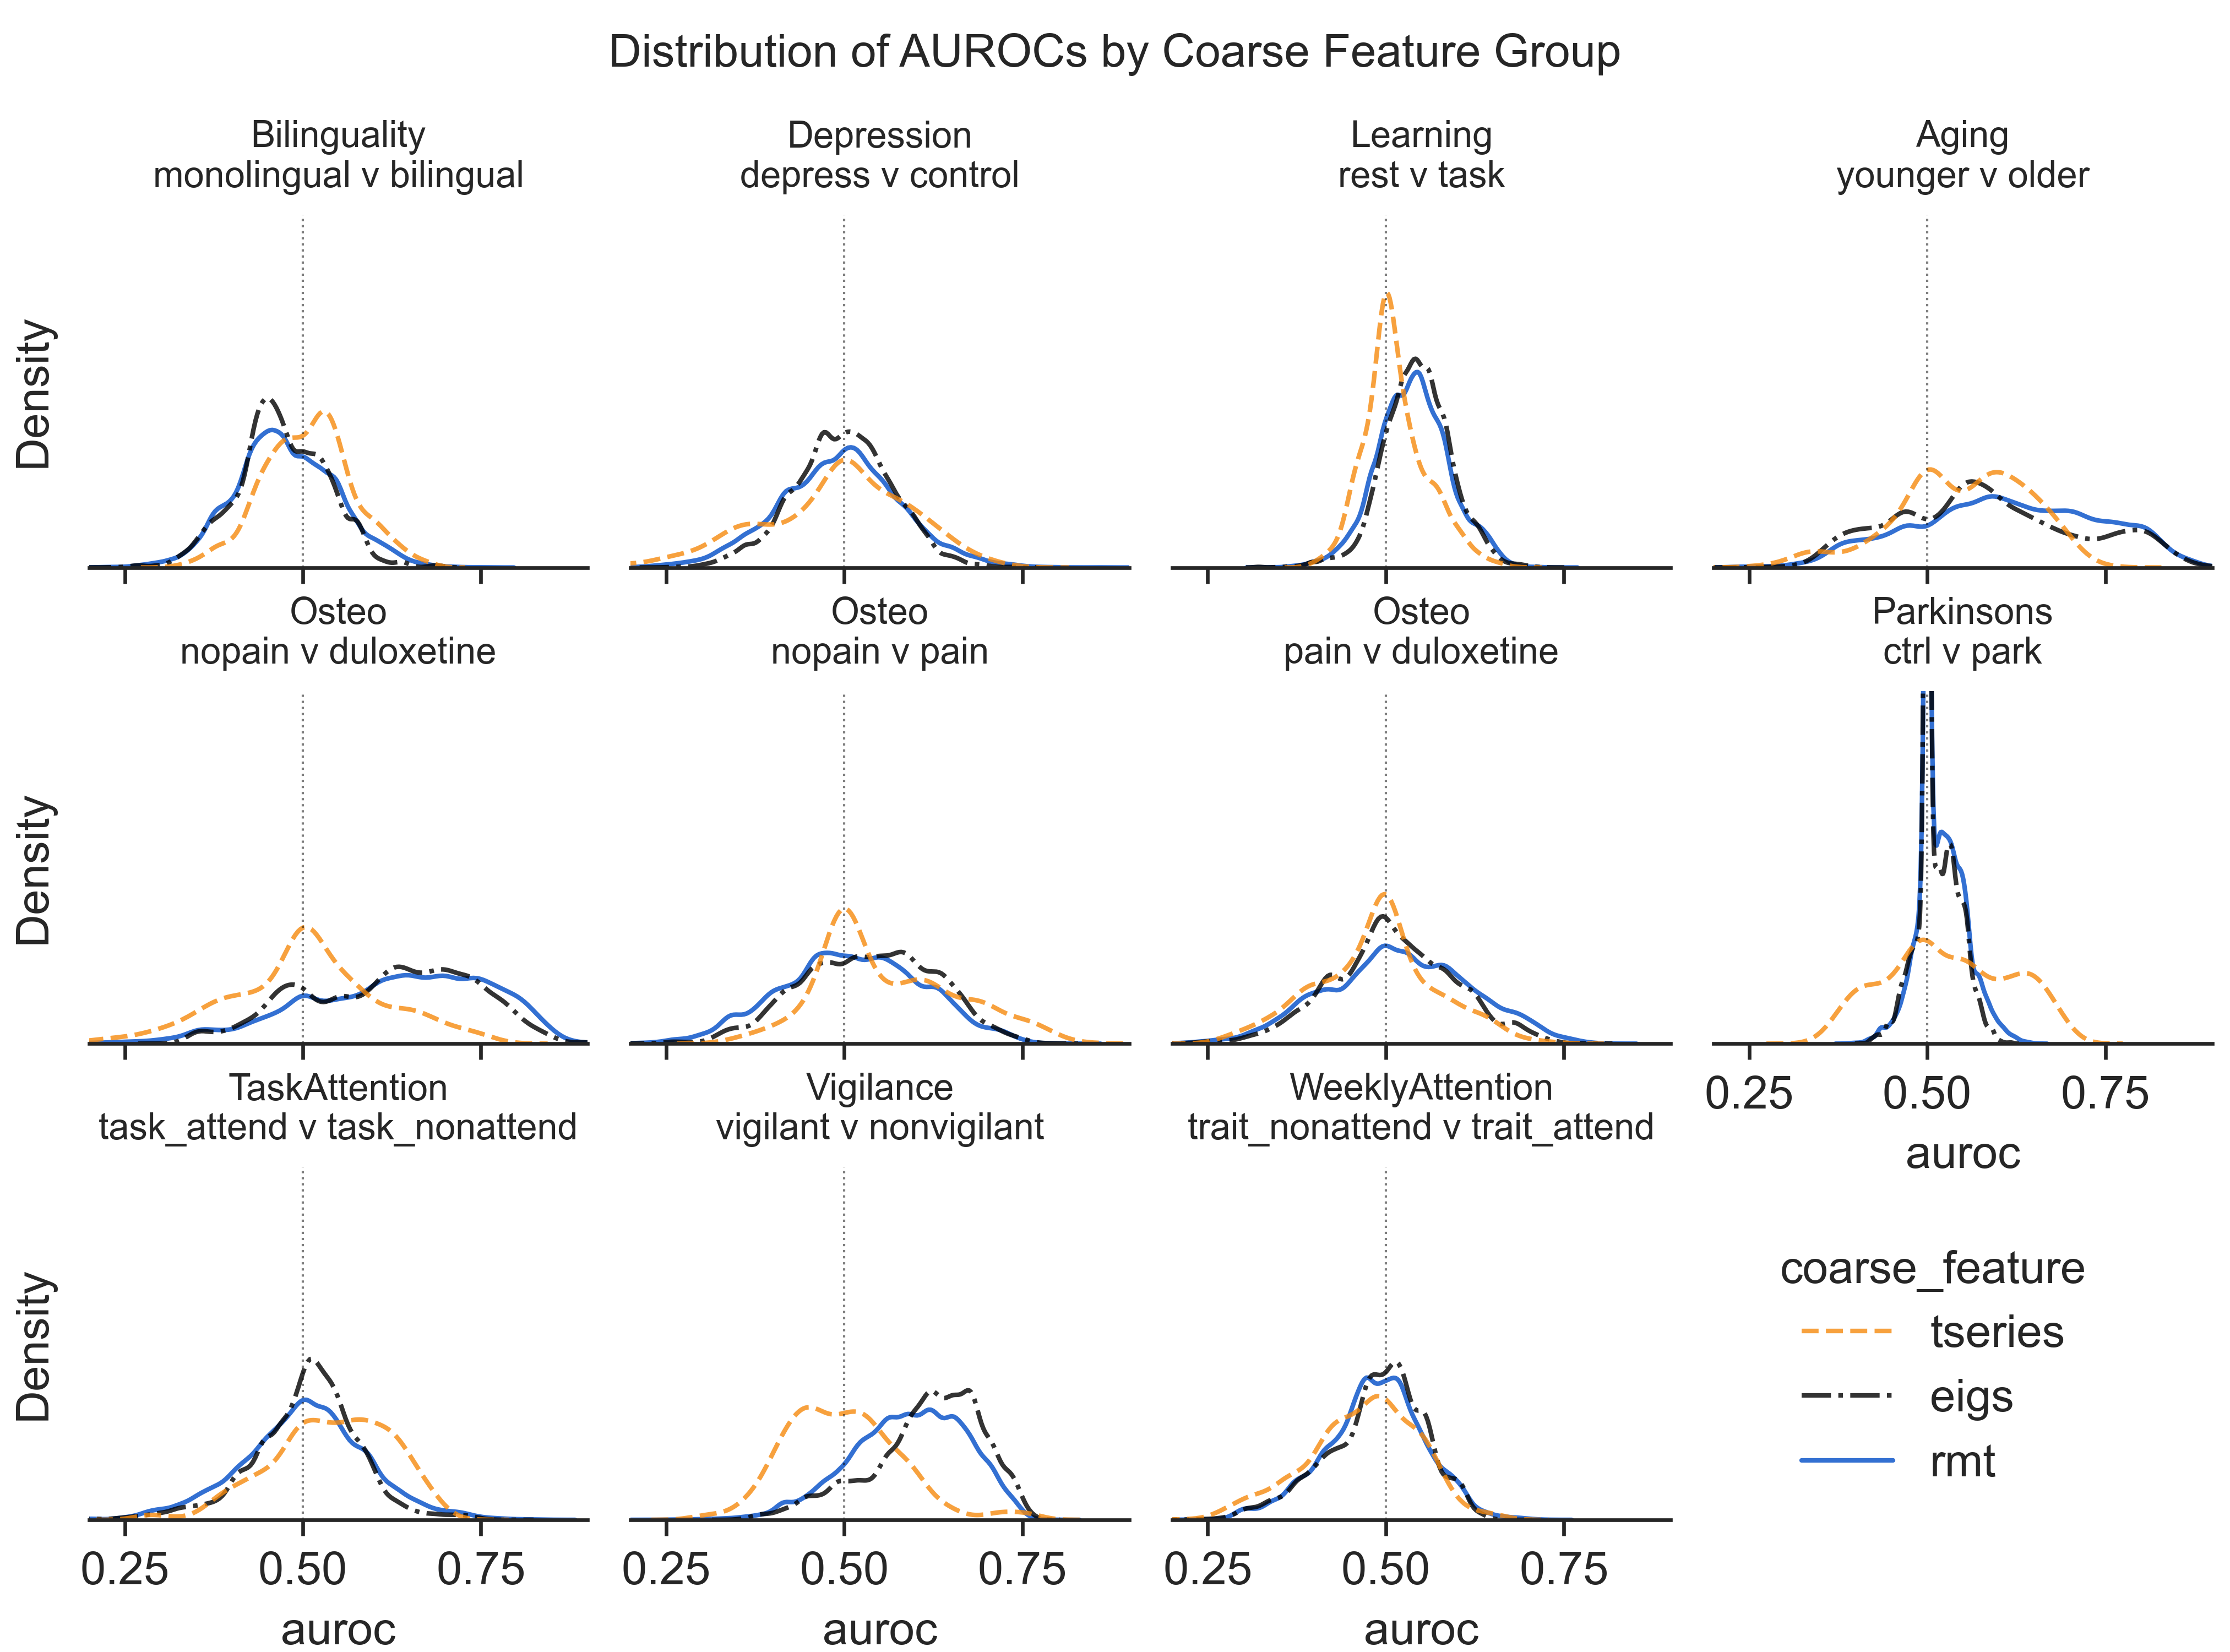
\includegraphics[width=6.5in]{coarse_feature_overall_by_subgroup.png}
\end{tabular}
\end{center}
\caption
{ \label{fig:main-results}
AUROC distributions across gross feature groupings and comparison tasks.}
\end{figure}

\subsection{Classification Tasks}

\subsubsection{Non-Predictable Comparisons}

It is important, to reduce figure clutter and complexity, to exclude a
classification task or an analytic factor from summaries if there is no
evidence that the classification task is solvable in general, or if, when
restricting the analytic factor to a particular instance, there is no evidence
of solvability. \textcolor{orange}{For example,} if a particular trimming
procedure were to render all classification tasks unsolvable, it would be
better to note this and exclude the associated mAUROCs from further
visualizations, rather than to have the mAUROC distributions diluted by the bad
procedure.

We take as lack of evidence of solvability an mAUROC distribution that is
either (1) roughly symmetric and has mean and median close to 0.5, i.e.
performance appears random, or (2) with median and mode less than 0.5. Based on
the mAUROC distributions for either coarsely-grouped (Figure
\ref{fig:main-results}) or finely-grouped features (Figure
S\ref{S-fig:feature-group-all}), neither bilinguality nor depression were
predictable by either baseline or eigenfeatures. Additionally, the \code{pain v
duloxetine} comparison in the \textit{Osteo} dataset, and the
\code{trait\_attend v trait\_nonattend} conditions ("WeeklyAttend" in Figures
\ref{fig:main-results} and S\ref{S-fig:feature-group-all}) in the
\textit{Attention} dataset were also not meaningfully predictable by any
feature. As such, we exclude these classification tasks from further figures
and discussion. We did not, however, find that any analytic factor resulted in
unsolvability.


\subsubsection{Predictable Comparisons}
As visible in Figure \ref{fig:main-results}, when coarsely summarizing
features, eigenfeatures were more likely to be predictively useful than not,
and except for in the \code{task\_attend v task\_nonattend} comparison, were
also more predictively useful than the baseline features.  Eigenfeatures most
strongly and consistently demonstrated predictive utility in the \textit{Aging}
dataset \code{older v younger} classification task, the \textit{Osteo} dataset
\code{nopain v duloxetine} task, and in the \textit{Attention} \code{vigilant v
nonvigilant} comparison.


\subsection{Largest mAUROCs}
\label{sec:unfolding-importance}
Considering the various analytic choices as tunable parameters, it makes sense
to examine the \textit{largest} portion of mAUROCs as an indication of the
maximum predictive potential of the eigenfeatures. In this case, it is clear
that eigenfeatures using RMT features almost always had the highest potential
predictive utility (Figure \ref{fig:largest}). Figure S\ref{S-fig:fine-largest}
shows that this was primarily due to either the "rmt only" or "rmt + eigs"
features (see Table \ref{tab:features}). However, RMT eigenfeatures were also
most likely to cause poor performance and overfitting (indicated by an mAUROC
\(<\) 0.5; Figure S\ref{S-fig:fine-smallest}).

Examining these RMT features more closely, it is clear these features'
performance distributions differ mostly due to the unfolding procedure. That
is, combined features that used the unfolded eigenvalues plus some other RMT
eigenfeature tended to have visually-indistinguishable mAUROC distributions to
those using the unfolded eigenvalues alone (Figures
S\ref{S-fig:fine-trim}-\ref{S-fig:fine-degree}). Instead, the mAUROC
distributions of these features differed mostly in the tails (Figures
S\ref{S-fig:fine-largest}-\ref{S-fig:fine-smallest}).


\begin{figure}
\begin{center}
\begin{tabular}{c}
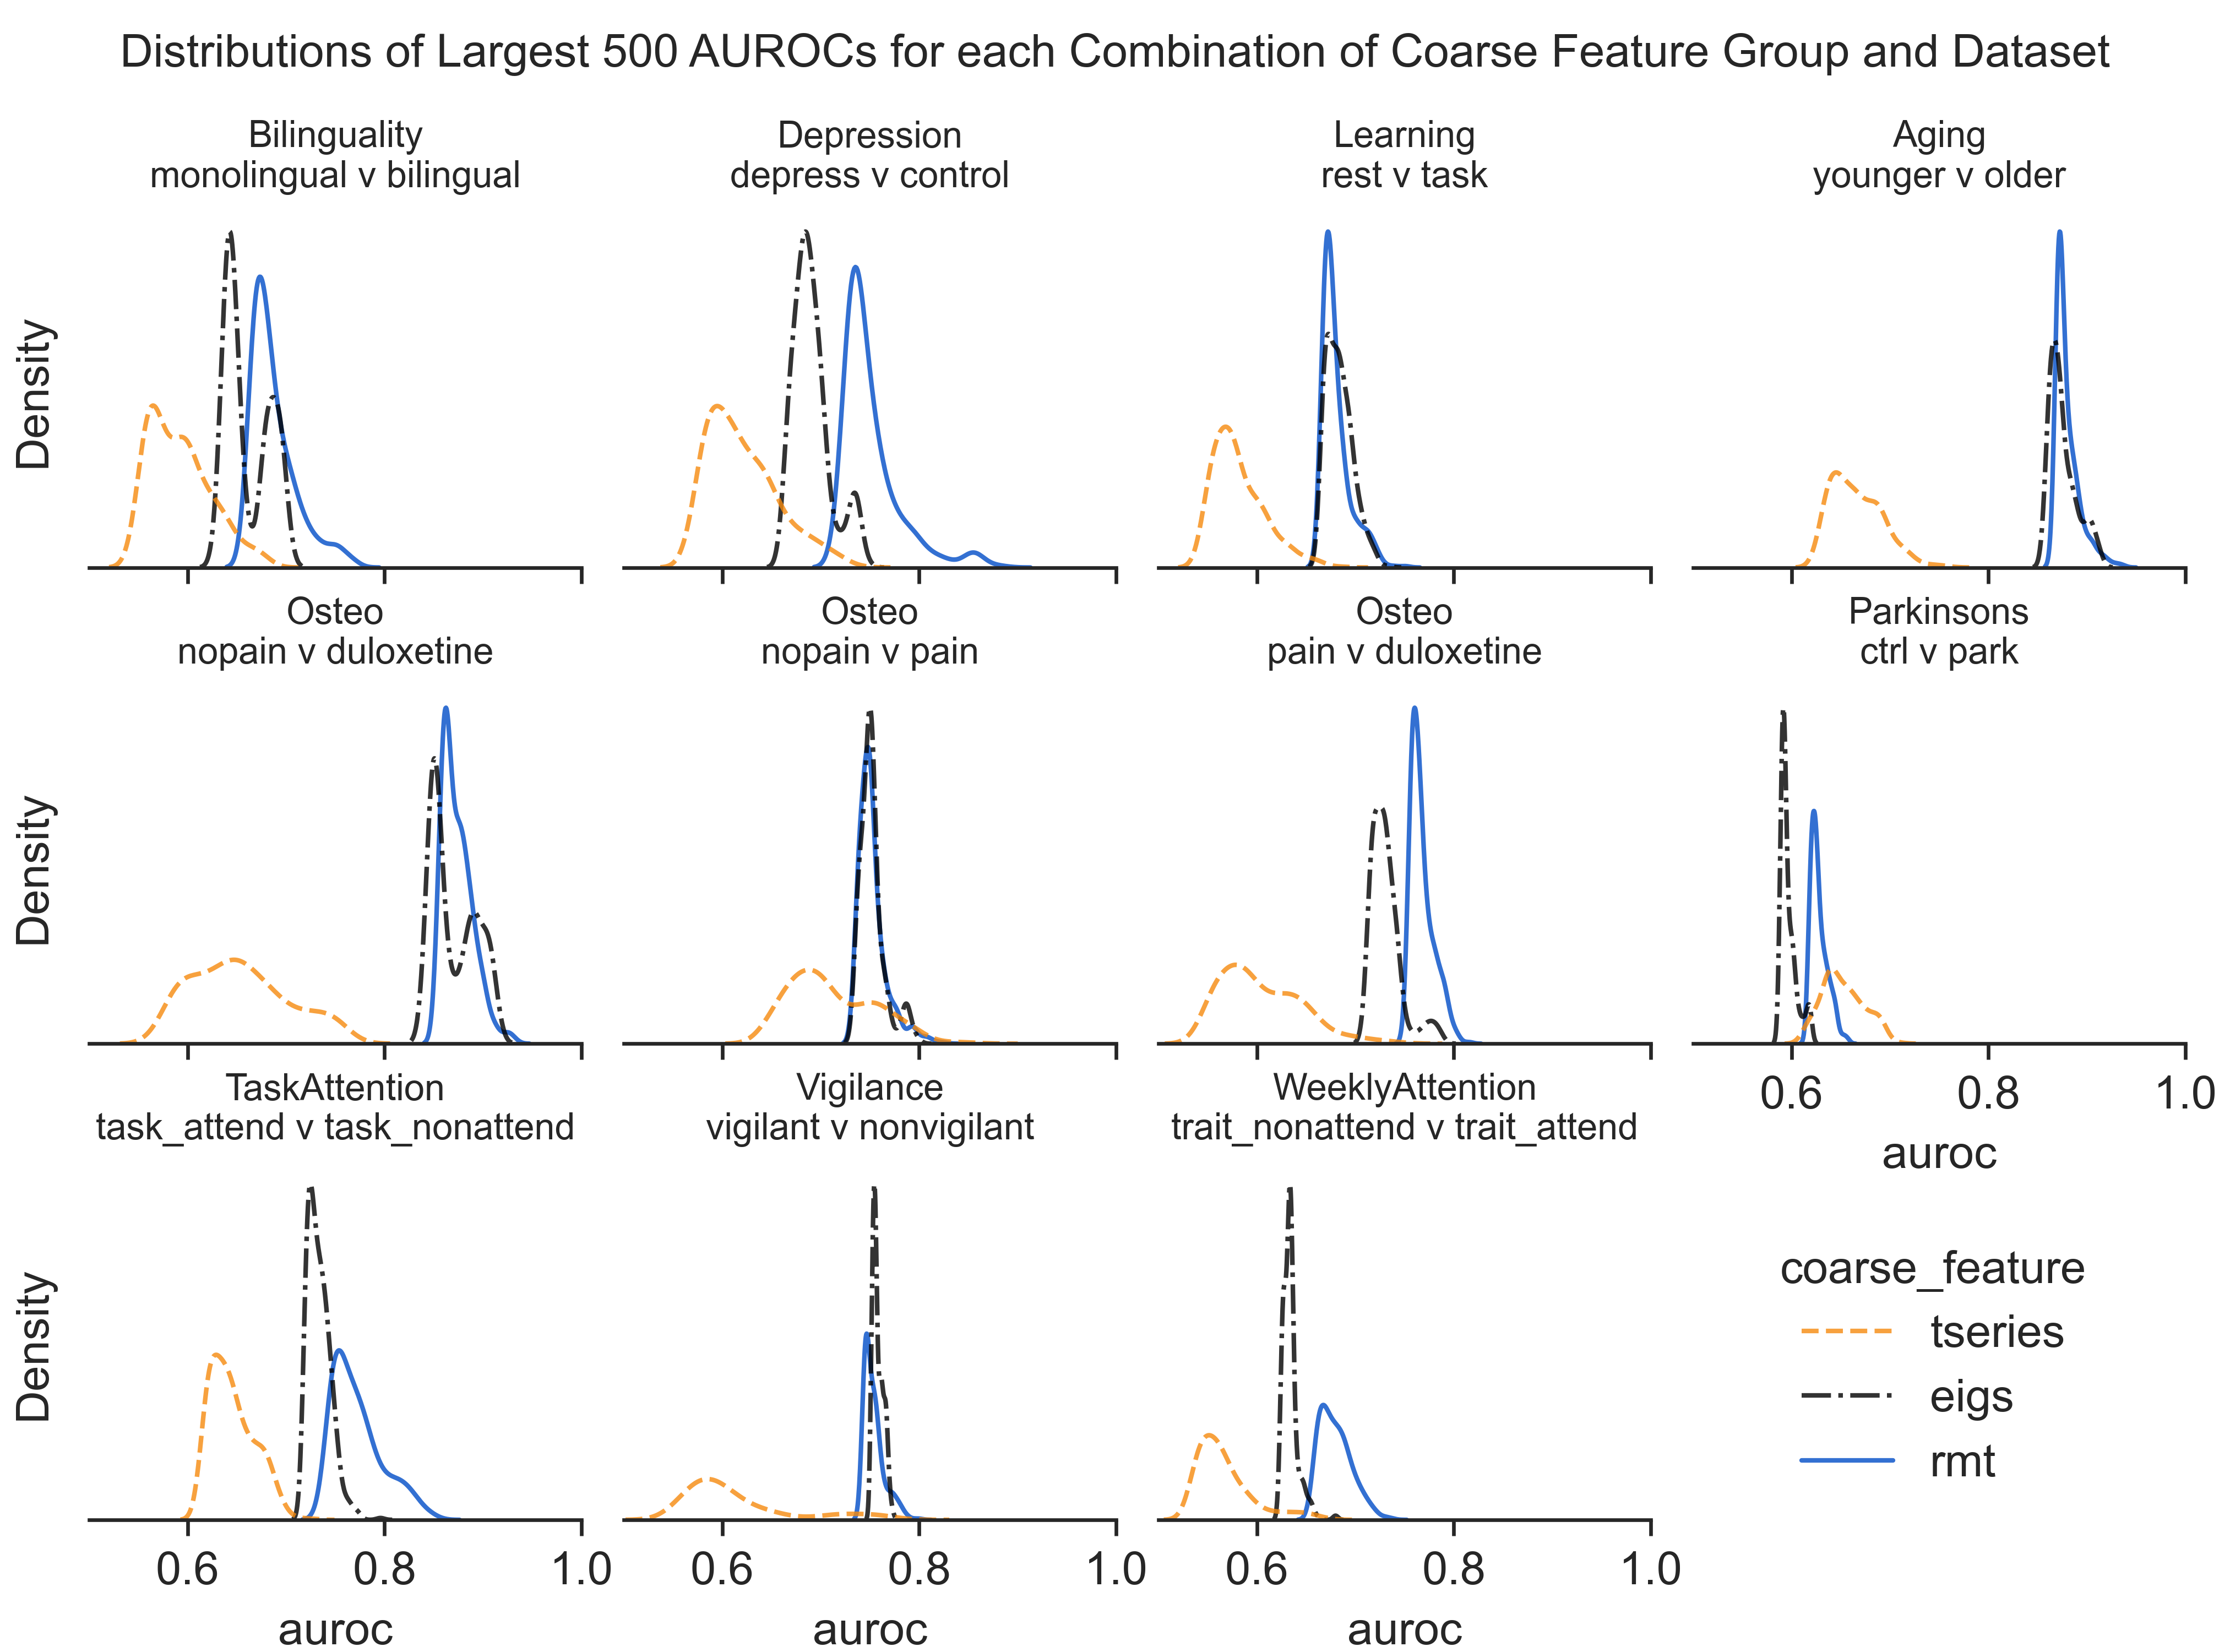
\includegraphics[width=6.5in]{coarse_feature_largest_by_subgroup.png}
\end{tabular}
\end{center}
\caption
{ \label{fig:largest} Distributions of largest 500 mAUROCs by coarse feature grouping.}
\end{figure}

\subsection{Effect of Preprocessing}
At a coarse level of feature grouping, slice time correction followed by motion
correction tended to slightly increase the predictive utility of the
eigenfeatures (Figure \ref{fig:preproc}) relative to brain extraction only.
Subsequent registration following these steps did not generally impact mAUROC
distributions further, except in the \code{task\_attend v task\_nonattend}
comparison, where registration reduced the predictive utility of the
eigenfeatures (Figure \ref{fig:preproc}, second-last column). When examining
features more finely, it is clear that preprocessing most impacts the mAUROC
distribution of the largest and central eigenvalues ("eigs middle" and "eigs
max" in Figure S\ref{S-fig:fine-preproc}).


\begin{figure}
\begin{center}
\begin{tabular}{c}
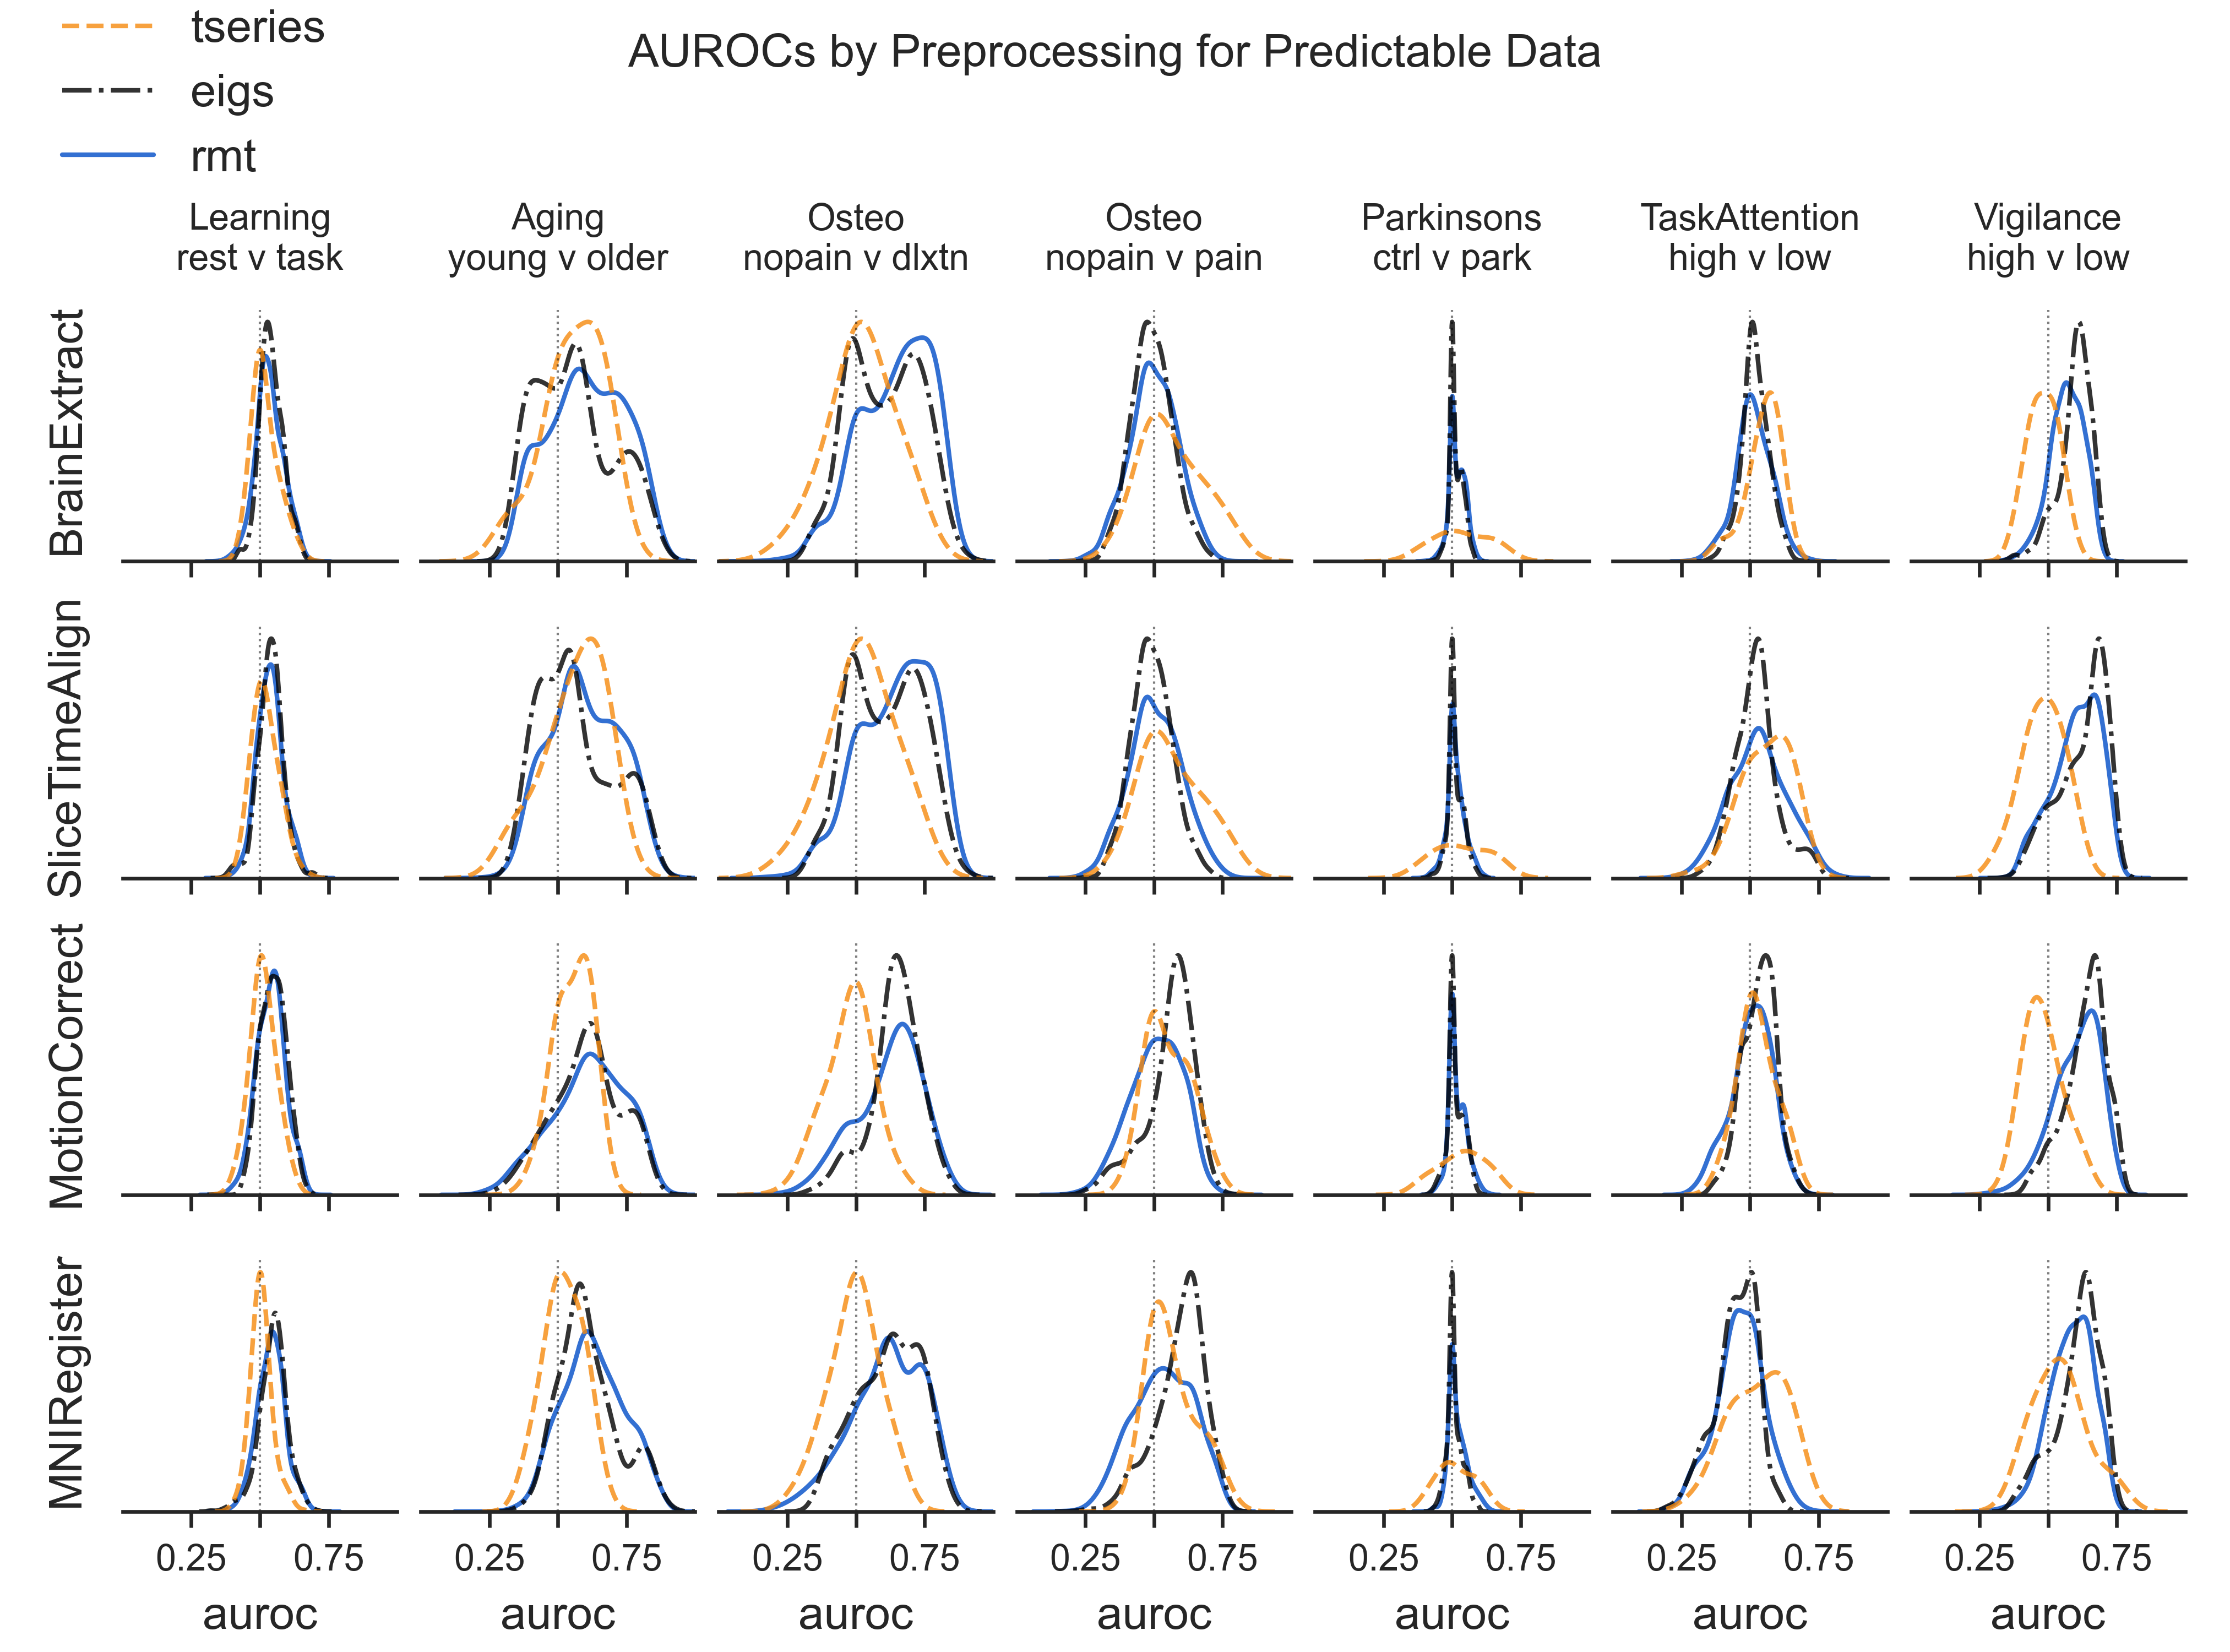
\includegraphics[width=6.5in]{coarse_feature_by_preproc_predictive_subgroup.png}
\end{tabular}
\end{center}
\caption
{ \label{fig:preproc} mAUROC distributions by preprocessing degree.}
\end{figure}

\subsection{Effect of Classifier}
Within any feature grouping (coarse or fine), and within a classification task,
mAUROC distributions were generally similar across classifiers (Figure
S\ref{S-fig:coarse-classifier}, S\ref{S-fig:fine-classifier}). Additionally,
these figures also show that within each classification task, choice of
classifier does not result in dramatic changes to the rough rank ordering of
features. E.g. if features are ranked on predictive utility, using the median,
modal, or bulk of the  mAUROC values, this rank ordering appears to remain
similar across classifiers.

In the \textit{Attention} \code{task\_attend v task\_nonattend} condition,
eigenfeatures were modally predictive only with the random forest classifier,
whereas in the \textit{Aging} data, a SVC was least likely to have mAUROC \(<\)
0.5. Overall, however, differences in the mAUROC distributions due to
classifier were small and inconsistent.

\subsection{Normalization}
There was no visible effect of feature normalization on mAUROC distributions.


\subsection{Effect of Trimming}
Trimming based on numerical precision (see Section \ref{sec:rmt-features} and
Appendix \ref{sec:trimming}), did not result in meaningfully different mAUROC
distributions in any case (Figure S\ref{S-fig:fine-trim}). However, trimming
away the largest, or both largest and smallest eigenvalues, generally had a
significant positive effect on the predictive quality of RMT features, most
especially for RMT features involving the unfolded eigenvalues. When employing
these trimming methods, these features were consistently more predictive than
not (Figure S\ref{S-fig:fine-trim}).

\subsection{Effect of Unfolding Degree}
The choice of polynomial unfolding degree significantly impacted the mAUROC
distributions for most classification tasks and most RMT features, and most
significantly for the level variance features (Figure
S\ref{S-fig:fine-degree}). Overall, Figure S\ref{S-fig:fine-degree} weakly
suggests that either smaller (degree = 3) or larger (degree = 9) unfolding
degrees tend to yield the most predictively useful RMT features. However, when
restricting to the most predictive RMT features (those including the unfolded
eigenvalues), it seems clear from Figure S\ref{S-fig:fine-degree} that the
largest unfolding degree of 9 produces the most favourable mAUROC
distributions.

\subsection{Effect of Slicing}
The best slice size and location depended complexly on the classification task
and feature, and few general summaries can be made of these interactions.
However, features including the full spectrum (e.g. raw eigenvalues, smoothed
eigenvalues, and their combinations with RMT eigenfeatures) were slightly more
predictive when using the largest portions ("max-XX", rows in Figure
S\ref{S-fig:best-params-slicing}), and usually least predictive when features
primarily involved the smallest or central portions.

\subsection{Choice of Summary Metric}
We note briefly that most of the above findings regarding the impacts of
analytic factors, and rank ordering of feature predictive utilities, are
similar when using the adjusted accuracy (see Section \ref{sec:multiverse}),
instead of the mAUROC (see Figures
S\ref{S-fig:feature-group-all-acc}-\ref{S-fig:best-params-slicing-acc}).
However, if comparison task predictability is defined as requiring adjusted
accuracies to be more positive than negative, then the \textit{Learning} and
\textit{Parkinson's} datasets do not appear to be predictable with any feature
(Figure S\ref{S-fig:feature-group-all-acc}).


\section{Discussion}
\label{sec:discussion}

In this study, eigenfeatures inspired by RMT and derived from the eigenvalues
of the full, whole-brain voxelwise fMRI correlation matrix were found to have
predictive utility across a wide variety of phenomena and analytic choices.
Compared to simple baseline reductions of the fMRI data, these eigenfeatures
had more consistent predictive utility, and a higher maximum predictive
potential (Figures \ref{fig:main-results}-\ref{fig:largest}). In addition to
evidence from previous studies \cite{sebaRandomMatrixAnalysis2003,
wangRandomMatrixTheory2016, matharooSpontaneousBackpainAlters2020}, this
suggests RMT may be a useful analytic and theoretical tool for understanding
functional connectivity.

However, eigenfeature mAUROC values observed in this study were highly
sensitive to the overall analytic procedure, and there was no single analytic
choice (e.g. choice of trimming procedure, unfolding polynomial degree, number
of preprocessing steps, or feature slicing) that ensured, for any combination
of feature and classification task, that all other analytic choices resulted in
mAUROC values greater than 0.5. In addition, the mean, median and modal mAUROCs
were generally close to 0.5, and adjusted mean and median accuracies also
tended to be close to zero. Thus we find limited evidence that
functional-connectivity-based eigenfeatures have general, "out of the box"
predictive utility, with general utility likely requiring either careful
tuning, or different preprocessing decisions and analytic choices than those
examined here.



\begin{table}[h!]
\caption{
\label{tab:top3-fine}
Top three robust maximum (\(95^{\text{th}}\) percentile) mAUROC and adjusted
accuracy (acc+) values for each predictable classification task and fine
feature grouping, sorted by mAUROC. A dash indicates that the fine feature
grouping for that row was not in the top three, i.e., that the top three
performing features differed depending on the performance metric. }
\small
\centering
\begin{tabular}{llcc}
\hline
                                   &               & mAUROC &   acc+ \\
Classification Task                & Source Feature&        &        \\
\hline
Aging - younger v older            & eigs smooth   &  0.834 &  0.226 \\
                                   & rmt + eigs    &  0.828 &  0.212 \\
                                   & eigs          &  0.823 &  0.211 \\
Learning - rest v task             & rmt + eigs    &  0.638 &  0.007 \\
                                   & eigs          &  0.636 &  0.007 \\
                                   & eigs max      &  0.631 &    –   \\
                                   & eigs middle   &    –   &  0.012 \\
Osteo - nopain v duloxetine        & rmt only      &  0.819 &  0.259 \\
                                   & eigs max      &  0.812 &  0.226 \\
                                   & rmt + eigs    &  0.806 &    –   \\
                                   & eigs smooth   &    –   &  0.212 \\
Osteo - nopain v pain              & tseries loc   &  0.762 &  0.104 \\
                                   & tseries scale &  0.697 &    –   \\
                                   & eigs smooth   &  0.684 &    –   \\
                                   & eigs middle   &    –   &  0.069 \\
                                   & eigs          &    –   &  0.034 \\
Parkinsons - ctrl v park           & tseries scale &  0.687 &  0.107 \\
                                   & tseries loc   &  0.657 &  0.063 \\
                                   & rmt only      &  0.590 &  0.027 \\
TaskAttention - task\_attend v task\_nonattend     & tseries loc &  0.666 &
0.135 \\
                                   & rmt only      &  0.660 &  0.121 \\
                                   & tseries scale &  0.656 &  0.124 \\
Vigilance - vigilant v nonvigilant & eigs middle   &  0.733 &  0.184 \\
                                   & eigs smooth   &  0.726 &    –   \\
                                   & rmt + eigs    &  0.719 &  0.162 \\
                                   & eigs          &    –   &  0.162 \\
\hline
\end{tabular}
\end{table}


Nevertheless, in all datasets, there were combinations of analytic choices that
resulted in cross-validated mean prediction performances well beyond mere
guessing (Figures S\ref{S-fig:fine-largest}, S\ref{S-fig:fine-largest-acc},
Table \ref{tab:top3-fine}). Whether or not these should be considered to have
practical relevance depends on one's goals, however, we note that with small
datasets of rs- or task-fMRI data, binary, subject-level classification using
whole-brain features is generally challenging.

For example, deep learning methods improve upon guessing by 17\% for autism
\cite{bengs4DSpatioTemporalDeep2020} or 3-30\% for ADHD
\cite{riazDeepFMRIEndtoendDeep2020}, 16\% for severe depression
\cite{ramasubbuAccuracyAutomatedClassification2016}, and 23\% for obsessive
compulsive disorder \cite{takagiNeuralMarkerObsessiveCompulsive2017}. Manual
feature engineering with more separable conditions (e.g. schizophrenia) can
result in classification accuracies well above 90\%
\cite{duHighClassificationAccuracy2012}, and with larger data, sophisticated
custom feature extraction methods can achieve near perfect accuracies at
classifying task vs. rest
\cite{zhangCharacterizingDifferentiatingTaskbased2016}. However, for functional
connectivity data and with classical machine learning algorithms (such as SVC)
we in general only expect large prediction accuracies (e.g. greater than 80\%)
when the group functional connectivities are already strongly separated (e.g.
Cohen’s \(d > 1.0\))\cite{dansereauStatisticalPowerPrediction2017}. In this
study, the (robust) maximum improvements upon guessing are shown in Table
\ref{tab:top3-fine}, and vary from 3-26\%.

It is somewhat surprising that the eigenfeatures examined here ever have net
cross-validated predictive utility. The reduction of the functional
connectivity matrix to the sorted \(t - 1\) eigenvalues uses all brain voxels
(including grey matter voxels), and destroys a large amount of information
(radically different matrices can have identical sorted eigenvalues). The
subsequent small-degree polynomial fit used in the unfolding procedure further
reduces variance in the raw data, and all eigenfeatures, due to the eigenvalue
sorting, are monotonically increasing curves (or approximately monotonic). All
such curves could likely be fit near-perfectly with 3-5 parameters, i.e. the
inherent dimensionality of these features is quite small. Interpreting the
eigenvalues as the magnitudes of the principal components of the standardized
data, this suggests that a rough summary of the magnitudes of the principal
components can often be surprisingly predictive in fMRI.

We speculate that the unfolded eigenvalues may have predictive utility in part
because of their smoothing and re-scaling effect (see also Section
\ref{sec:unfolding-importance}). Figure \ref{fig:unfolded}, which depicts the
raw eigenvalues and unfolded eigenvalues with different trimming procedures,
shows how the raw eigenvalues have strongly exponential distributions, even
with logarithmic axes. This is due to the magnitude of the largest eigenvalues,
and the unfolded and trimmed feature distribution in Figure \ref{fig:unfolded}
are far less pathologically distributed.

\begin{figure}
\begin{center}
\begin{tabular}{c}
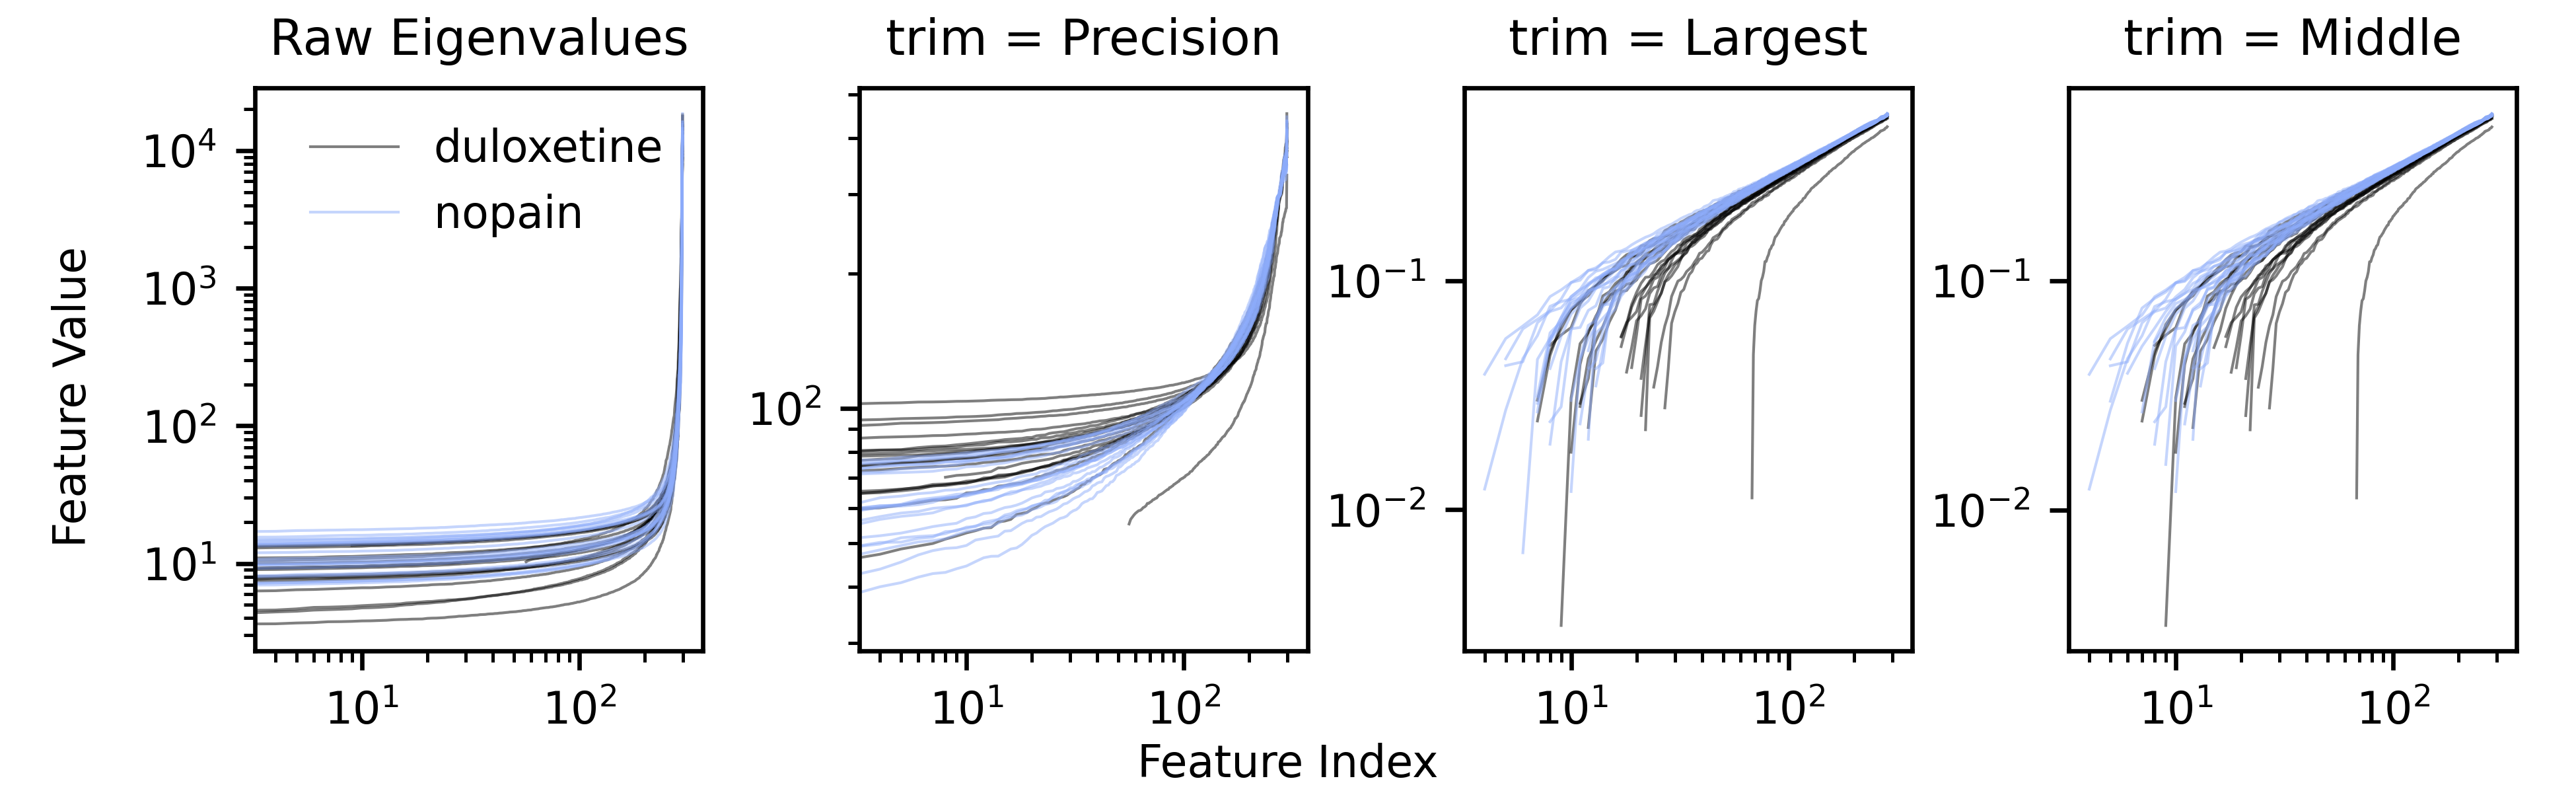
\includegraphics[width=6.5in]{unfolded_osteo_duloxetine_v_nopain.png}
\end{tabular}
\end{center}
\caption
{ \label{fig:unfolded} Raw eigenvalues (first subplot) and unfolded eigenvalues
(polynomial degree 9; last 3 subplots) for \textit{Osteo} dataset
\footnotesize\texttt{duloxetine v nopain} classification task, brain extraction
and slice time correction only. Median observed mAUROC = 0.643 (range = 0.346 -
0.925)}
\end{figure}

% It was also sometimes the case that adding RMT-specific features (e.g. the
% spectral rigidity, or level variance) to either the unfolded or raw
% eigenvalues would allow for a higher maximum mAUROC (Tables
% \ref{tab:numerical}-\ref{tab:top3-fine}, and Figure
% S\ref{S-fig:fine-largest}). One case where these features yielded the largest
% predictions was in the \textit{Aging} dataset. This is depicted in Figure
% \ref{fig:observables}, where it is clear that, after trimming, at almost any
% \(L\) value, subgroups either cluster in bands, or tend to generally have
% lower or higher rigidity of level variance curves.

% \begin{figure}
% \begin{center}
% \begin{tabular}{c}
% 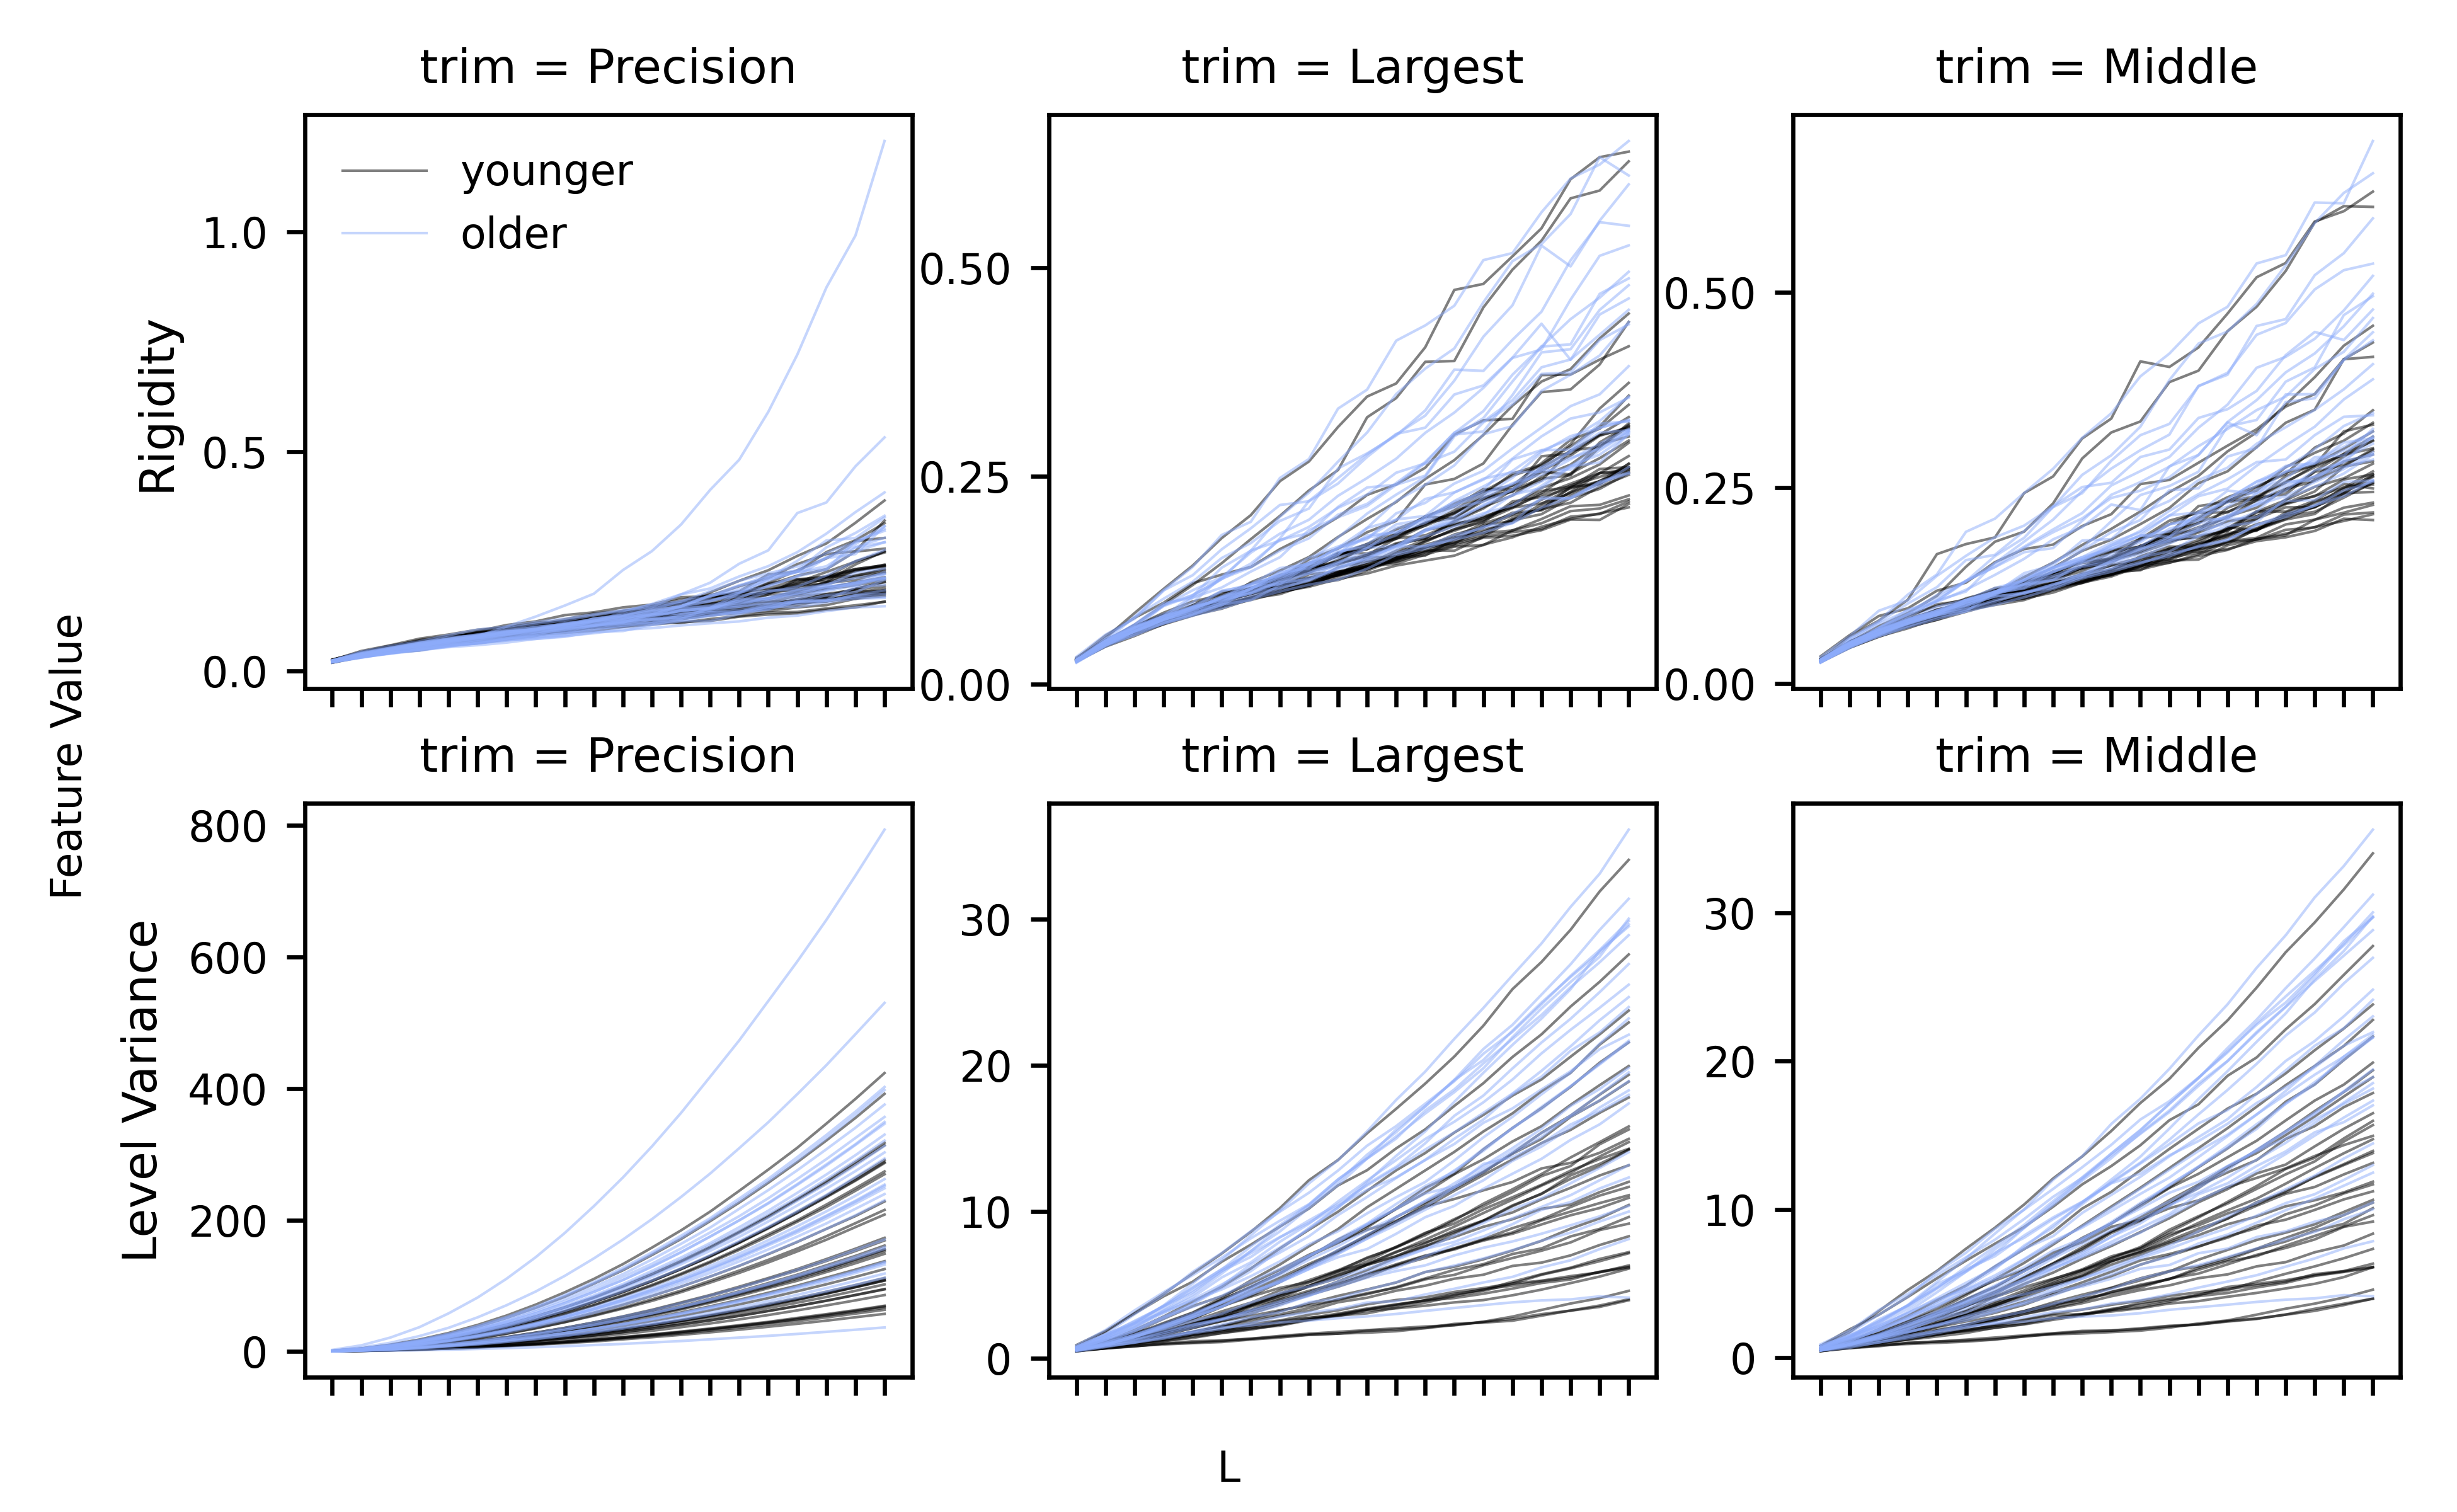
\includegraphics[width=6.5in]{observables_older_younger_v_older.png}
% \end{tabular}
% \end{center}
% \caption
% { \label{fig:observables} Rigidity and level variance features (unfolding
% polynomial degree 3) for \textit{Aging} dataset \footnotesize\texttt{younger v
% older} classification task, brain extraction only. Median observed mAUROC =
% 0.703 (range = 0.424 - 0.880). Horizontal axis L-values range from 1 to 20 in
% all subplots, as described in Section \ref{sec:methods}. Note banding / clusters
% related to classes.}
% \end{figure}

\subsection{Limitations}
As is unfortunately typical of fMRI research\cite{turnerSmallSampleSizes2018},
the number of subjects in each dataset was quite small (Table
\ref{tab:data-subjects}). With such small numbers of subjects, randomization
cannot be expected to effectively control group differences, and it is possible
the predictive utility of the eigenfeatures was due to capitalization of such
differences. For example, eigenfeatures were generally predictive in the
\textit{Aging} dataset, and it is quite possible for randomization failures to
introduce age imbalances across classes.

Likewise, one of the other more predictable classification tasks was the
\code{duloxetine v nopain} task in the osteoarthritis dataset. An active drug
could introduce any number of physiological confounds relevant to
fMRI\cite{murphyRestingstateFMRIConfounds2013}, but we could not control for
such effects do to the absence of physiological recording in most datasets.

In general, much larger fMRI datasets are needed to adequately control for and
test \textit{what} exactly the connectivity eigenvalues actually predict, and
to test if these predictions generalize to larger, different populations.



\section{Conclusion}

Eigenvalue-based features inspired by RMT, and extracted from fMRI functional
connectivity matrices were found to have predictive utility across a wide
variety of datasets and classification tasks. However, the predictive utilities
were modest, and highly dependent on preprocessing steps and other fitting and
feature selection procedures.

\color{cyan}
Previous studies have not explored the sensitivity of RMT-based analyses to
analytic decisions. It is far too early to say whether RMT may prove fruitful
for understanding fMRI, however, we hope our analyses show that, \textit{if}
RMT has such potential, that potential must be contextualized by the analytic
decisions involved. Absent this context, we advise caution with regard to
claims that RMT offers insights into fMRI analyses.


\color{black}


Future studies employing RMT should carefully
investigate the sensitivity of any findings to such analytic decisions before
drawing any conclusions. However, this study demonstrates that the inclusion of
RMT statistics and other eigenfeatures extracted from fMRI images could aid in
the predictive modeling of a wide variety of phenomena.



\newpage



\section*{Disclosures}
JL is founder of Time Will Tell Technologies, Inc.. The authors have no
relevant financial interests in the manuscript and no other potential conflicts
of interest to disclose.



\section*{Acknowledgments and Funding}
This work was supported by the Natural Science and Engineering Research
Council of Canada's Canada Research Chair grant (grant number 231266) to JL,
Natural Science and Engineering Research Council of Canada Discovery Grant to
JL, a Canada Foundation for Innovation and Nova Scotia Research and Innovation
Trust infrastructure grant (R0176004) to JL, a St. Francis Xavier University
research startup grant to JL (grant number R0168020), and a St. Francis Xavier
University UCR grant to JL.



\section*{Data, Materials, and Code Availability}
\label{sec:data-and-code}

All raw fMRI data used in this study is publicly available on the
\href{https://openneuro.org/}{OpenNeuro}
platform\cite{poldrackOpenfMRIOpenSharing2017,
markiewiczOpenNeuroResourceSharing2021}.

All code used specifically to perform preprocessing and analyses for this paper
is publicly available
\href{https://github.com/DM-Berger/random-matrix-fmri/}{online} in the paper
GitHub repository\cite{dm-bergerDMBergerRandommatrixfmriPaper2022}. This
repository also includes all produced prediction data in a single table
available in the file \code{all\_produced\_prediction\_data.json.xz} available
\href{https://github.com/DM-Berger/random-matrix-fmri/blob/master/all\_produced\_prediction\_data.json.xz}{in
the paper repository}.

Code used to compute the spectral observables and perform unfolding is publicly
available in the
\href{https://github.com/stfxecutables/empyricalRMT}\code{empyricalRMT}
library\cite{dm-bergerStfxecutablesEmpyricalRMTV12022}.



\newpage



\appendix

\section{Correlation Eigenvalues via Transposition}
\label{sec:transpose}

Let \(\mathbf{X}\) be a real \(n \times p\) matrix with \(n > p\). Let
\[
\mathbf{Z} = \text{norm}(\mathbf{X}) =
\left(
\mathbf{X}_1 - \bar{\mathbf{X}}_1 | \dots | \mathbf{X}_p - \bar{\mathbf{X}}_p
\right)
\]
where \(\mathbf{X}_i\) denotes column \(i\) of \(\mathbf{X}\). Denote the
(unordered) set of eigenvalues of \(\mathbf{X}\) as
\(\text{eigs}(\mathbf{X})\), and let \(r = (p - 1)^{-1}\). Denote the
covariance matrix of \(\mathbf{X}\) as \(\text{cov}(\mathbf{X})\).  Then:
\begin{align*}
\text{eigs}\left( \text{cov}(\mathbf{X})  \right)
&= \text{eigs}(r \cdot \mathbf{Z}\mathbf{Z}^{\top}) \\
&= r \cdot \text{eigs}(\mathbf{Z}\mathbf{Z}^{\top}) \\
&= r \cdot \text{eigs}((\mathbf{Z}\mathbf{Z}^{\top})^{\top}) \\
&= r \cdot \text{eigs}(\mathbf{Z}^{\top}\mathbf{Z}) \\
\end{align*}

Denote the correlation matrix of \(\mathbf{X}\) as \(\text{corr}(\mathbf{X})\),
and let
\[
\mathbf{Y} = \text{standardize}(\mathbf{X}) =
\left(
(\mathbf{X}_1 - \bar{\mathbf{X}}_1) / \sigma_1 | \dots | (\mathbf{X}_p - \bar{\mathbf{X}}_p) / \sigma_p
\right)
\]
Then
\[
\text{eigs}\left( \text{corr}(\mathbf{X})  \right)
= \text{eigs}\left( \text{cov}(\mathbf{Y})  \right)
= r \cdot \text{eigs}(\mathbf{Y}^{\top}\mathbf{Y})
\]

\section{Trimming Procedures}
\label{sec:trimming}

We implement three trimming procedures: precision-based, largest, and middle
trimming. The
\href{https://github.com/DM-Berger/random-matrix-fmri/blob/7c9e4187f582dedee728cd7193b8894d928c2f00/code/rmt/updated_dataset.py#L431-L444}{source
code} is the definitive reference for the procedures, but we describe the
motivations belows.

In precision-based trimming, we trim away any eigenvalues that are close enough
to zero to be considered a result of numerical error due to floating point
representation. There are two thresholds we consider, including the one used by
NumPy\cite{harrisArrayProgrammingNumPy2020} for the
\href{https://numpy.org/doc/stable/reference/generated/numpy.linalg.matrix_rank.html}{determination
of matrix rank}, and those recommended by LAPACK\cite{laug} in their user
guide\cite{andersonLAPACKUsersGuide1999a} on the
\href{https://netlib.org/lapack/lug/node89.html}{error bounds for symmetric
eigenproblems}, and related
\href{https://netlib.org/lapack/lug/node90.html}{additional details}. We trim
each matrix eigenvalues to whichever threshold is largest for the matrix in
question.

For largest trimming, we must determine a threshold at which to separate
"large" from "small" eigenvalues. The eigenvalues for our data tended to grow
exponentially, so we instead looked at thresholding on the logarithms. We then
used \(k\)-means with \(k=2\) on the precision-trimmed eigenvalues, and took
the largest cluster (which also always had the smaller mean) cluster as the
"largest" eigenvalues to trim away. "Middle" trimming simply reflects the
threshold found by the largest trim method, e.g. if the largest trim method
removes the last \(n\) precision-trimmed eigenvalues, then we also trim the
first \(n\) smallest eigenvalues remaining after precision-trimming.

We chose one-dimensional k-means partly due to efficiency and simplicity, and
because of the general relation to classical thresholding methods like the Otsu
method\cite{liuOtsuMethodKmeans2009}.



%%%%% References %%%%%

\bibliography{report}   % bibliography data in report.bib
\bibliographystyle{spiejour}   % makes bibtex use spiejour.bst

%%%%% Biographies of authors %%%%%

% \vspace{2ex}\noindent\textbf{First Author} is an assistant professor at the University of Optical Engineering. He received his BS and MS degrees in physics from the University of Optics in 1985 and 1987, respectively, and his PhD degree in optics from the Institute of Technology in 1991.  He is the author of more than 50 journal papers and has written three book chapters. His current research interests include optical interconnects, holography, and optoelectronic systems. He is a member of SPIE.

\vspace{1ex}
\noindent Biographies and photographs of the other authors are not available.

\listoffigures
\listoftables

\end{spacing}
\end{document}